\section{Open versus Sealed Bidding in Timber Auctions: Athey, Levin and Seira (2011)}\label{sec:15-als}

This section studies one application from beginning to end. \citet{AtheyLevinSeira2011}, whom we
abbreviate ALS, ask whether a seller should sell by open ascending auction or by first-price sealed
bid. Their answer uses nearly every tool of this chapter. The sealed-bid model is the asymmetric
private values model, inverted through first-order conditions as in \cref{sec:15-gpv,sec:15-apv}.
Bids within an auction are correlated, so the model contains unobserved auction heterogeneity of the
kind studied in \cref{sec:15-uh}. Bidders choose whether to pay to participate, and entry costs are
recovered from an indifference condition as in \cref{sec:15-entry}. The equilibrium theory comes from
\cref{sec:14-asym,sec:14-entry,sec:14-collusion}. We follow the order of a full case study: question,
institutions, data, model, reduced-form evidence, structural estimation, validation, counterfactuals
and assessment.

\subsection{The question}\label{sec:15-als-question}

The choice between open and sealed bidding arises in sales of timber, oil leases, art, real estate and
financial assets, and in procurement. Theory identifies conditions under which either format is better
for efficiency or revenue. Evidence is scarce, because most markets operate under a single set of rules
\citep[p.~207]{AtheyLevinSeira2011}. ALS ask three questions. Which format attracts more bidders? Which
format raises more revenue? Does the allocation of the object depend on the rules?

The stakes are large in the timber market. Logging and milling form a \$100 billion a year industry in
the United States, and about 30 percent of timberland is publicly owned. During the period ALS study,
the federal government sold about \$1 billion of timber a year \citep[p.~208]{AtheyLevinSeira2011}.

Revenue equivalence (\cref{prop:14-ret}) is the benchmark. With risk-neutral bidders whose private
values are independent draws from one distribution, both formats yield the same expected revenue for a
fixed set of participants. The equivalence survives costly entry. If loggers and mills drew values from
the same distribution, the two formats would have the same expected entry, the same allocation and the
same expected revenue \citep[Section II.D]{AtheyLevinSeira2011}. Any systematic difference between the
formats must therefore come from a departure from the benchmark. Candidates include asymmetric bidders,
collusion, common values, correlated values and risk aversion.

Two departures pull in opposite directions. Sealed bidding favors weak bidders, because strong bidders
shade their bids more (\cref{prop:14-maskin-riley}, after \citealp{MaskinRiley2000}). Weak bidders then earn more from participating
and enter more often, an effect stressed by \citet{Klemperer2004}. The price of this advantage is an
inefficient allocation. The open auction allocates efficiently among participants, but a bidding ring
is self-enforcing in it (\cref{prop:14-robinson}). The first chief of the Forest Service, Gifford
Pinchot, chose sealed bids for that reason, ``thereby preventing the customary collusion between
bidders'' \citep[p.~209]{Pinchot1998}, as quoted by \citet[footnote 2]{AtheyLevinSeira2011}. A century
later, \citet[ch.~10, p.~207]{MarshallMarx2012} still list sealed instead of ascending bids first among
the measures an auctioneer can take against rings (\cref{sec:15-collusion}). Theory
gives no general revenue ranking, even with fixed participation \citep[p.~215]{AtheyLevinSeira2011}.
The comparison is quantitative, and it needs a model estimated from data.

The Forest Service timber program is a good test case. It uses both formats in the same forests, and
for some sales it chose the format at random \citep[p.~207]{AtheyLevinSeira2011}.

\subsection{Institutions}\label{sec:15-als-institutions}

A sale begins when the Forest Service identifies a tract of timber and organizes a \emph{cruise}, a
survey that estimates the merchantable timber on the tract. The sale is announced at least 30 days
before the auction. The announcement states the auction format, the estimated volume and logging
costs, the tract characteristics and a reserve price \citep[p.~218]{AtheyLevinSeira2011}. The reserve
price follows a formula. It starts from the cruise estimates of timber value and costs and adds a fixed
margin for profit and risk. Some sales are restricted to firms with fewer than 500, or fewer than 25,
employees. ALS exclude these small-business sales.

Before the auction, firms may cruise the tract themselves and prepare bids. The recording rules differ
by format \citep[p.~219]{AtheyLevinSeira2011}. In a sealed-bid sale the Forest Service records each
bidder's identity and bid. In an open auction each firm must submit a qualifying bid before the sale,
typically equal to the reserve price. The Forest Service records every qualifying firm and the highest
bid each one offers. Entry is therefore observed in both formats, including firms that never bid
actively in an open auction. Open auctions are conducted by outcry and the price can rise in jumps. ALS
know of no evidence that jump bidding mattered much, but it complicates inference from recorded open
bids \citep[footnote 3]{AtheyLevinSeira2011}, as \cref{thm:15-ht} makes precise.

After the auction the winner has a set period, typically one to four years in the sample, to harvest
the timber. In a \emph{scale sale} the winner pays per unit of timber removed, so revenue can
differ from the winning bid times the cruise volume. In a \emph{lump-sum sale} the winner pays the bid.
For scale sales ALS have limited harvest data and use the bid price as a proxy for revenue
\citep[p.~219]{AtheyLevinSeira2011}.

The format itself has a history \citep[pp.~210 and 221--226]{AtheyLevinSeira2011}. Sealed bidding
was used early in the twentieth century and has remained almost universal in the Southeast. Open
auctions gained favor elsewhere, especially in the Pacific Northwest, on the argument that they let
local mills respond directly to competition. In 1976 Congress mandated sealed bidding, but the
regulations allowed forest managers to use open auctions if they could justify the choice. The format
therefore continued to vary across places and times. \citet{SchusterNiccolucci1994} document from
interviews that for a subset of Northern sales the format was chosen at random. In some instances it
was decided by picking colored balls out of a sock (their p.~90, as cited by ALS, p.~226). ALS analyze
the 378 sales that Schuster and Niccolucci identify as randomized and obtain very similar estimates of
the effect of sealed bidding (reported in their Online Appendix).

\subsection{Data}\label{sec:15-als-data}

The unit of observation is a timber sale. The Northern sample covers sales held from 1982 to 1990 in the
Kootenai and Idaho Panhandle National Forests. These neighboring forests on the Idaho-Montana border have
the largest timber programs of the Forest Service's Northern region. The California sample covers sales
held from 1982 to 1989 \citep[p.~218]{AtheyLevinSeira2011}. In California the format varies more
systematically with sale size, which makes tract differences harder to control for. Prices are in 1982
dollars per thousand board feet of timber, abbreviated mbf.

For every sale ALS know the identity and bid of each participant and the characteristics in the sale
announcement. These include the reserve price and the Forest Service estimates of volume, selling value,
and logging, manufacturing and road-building costs. They also include the timber density, the contract
length, salvage and scale-sale indicators and a Herfindahl index of species concentration. Market conditions are measured
by monthly United States housing starts and county counts of logging firms and sawmills
\citep[p.~226]{AtheyLevinSeira2011}.

\casehead{Mills and loggers}
ALS classify bidders as \emph{mills}, which have manufacturing capacity, and \emph{loggers}, which do
not \citep[p.~219]{AtheyLevinSeira2011}. Other groupings, by number of employees or number of auctions
entered, turn out to be similar. The theory requires mills to be the stronger bidders, and the data agree.
A regression of log per-unit sealed bids on a mill dummy and auction fixed effects gives a coefficient
of 0.248 in the North, with a $t$-statistic of roughly 8 \citep[p.~220]{AtheyLevinSeira2011}. Mill bids
are thus about 25 percent higher than logger bids in the same auction. An entering mill wins more often
than an entering logger, 28 percent against 21 percent. In California mill bids are just over 12 percent
higher with auction fixed effects.

Two explanations for the mill advantage are cost differences and double marginalization. A logger who
wins must sell the logs to a mill, which may charge a margin over its processing costs. ALS give an
example \citep[footnote 10]{AtheyLevinSeira2011}. Suppose all bidders agree that the timber is worth
\$100,000 net of costs, and that a winning logger must pay a \$20,000 margin to one of two local mills.
Each logger values the contract at \$80,000. Each mill values it at \$90,000, since it expects to
collect the margin with probability one half if a logger wins.

Observed sale characteristics explain much of the variation in bids. Regressing individual log sealed
bids on sale characteristics and a logger dummy gives an $R^2$ of 0.62 in the North and 0.71 in
California. Regressing the average bid of each sale on sale characteristics gives 0.72 and 0.69
\citep[footnote 9]{AtheyLevinSeira2011}.

\casehead{Potential bidders}
The entry model needs the number of potential bidders of each type. For loggers, ALS count the distinct
logging companies that entered an auction in the same area over the previous year. The area is the forest
district in the North and the forest in California \citep[p.~221 and footnote 11]{AtheyLevinSeira2011}. The count contains measurement error, because firms enter and exit and bidder
names are recorded with varying spellings. For mills the model itself supplies the answer. In the
estimated equilibrium every potential mill enters, so the number of potential mills equals the number of
entering mills.

\casehead{Choice of format and trimming}
Format choice is related to observables, so ALS model it. A logit of a sealed-bid dummy on the sale
characteristics, potential-competition measures and dummies for year, quarter, location and species
gives their Table II. Sale size enters as a step function with 10 steps that roughly correspond to
deciles \citep[p.~227]{AtheyLevinSeira2011}. Smaller sales are more often sealed, and the effect is much
stronger in California. The coefficient on the largest volume category (over 90 hundred mbf) is $-2.479$
(s.e.\ 0.583) in the North and $-9.833$ (0.930) in California. The pseudo-$R^2$ is 0.19 in the North
($N=1{,}233$ sales) and 0.66 in California ($N=2{,}064$). Location dummies are jointly significant in
both regions (Table II).

The fitted probability of sealed bidding is the \emph{propensity score}. Some open sales look unlike any
sealed sale, and their propensity score is close to zero. ALS keep only sales with a propensity score
between 0.075 and 0.925 \citep[p.~227]{AtheyLevinSeira2011}. This drops 154 open and 8 sealed sales in
the North. In California it keeps only about one third of the sales: 707 of 2,064, by the counts in
their Table I. \Cref{tab:15-als-summary} reports the selected samples. They contain 1,071 Northern sales
(732 open, 339 sealed) and 707 California sales (325 open, 382 sealed).

\begin{table}[htbp]
\centering
\caption{Summary statistics for the selected samples (means, standard deviations in parentheses)}
\label{tab:15-als-summary}
\small
\setlength{\tabcolsep}{4pt}
\begin{tabular}{@{}lcccc@{}}
\toprule
 & \multicolumn{2}{c}{Northern forests} & \multicolumn{2}{c}{California forests}\\
\cmidrule(lr){2-3}\cmidrule(lr){4-5}
 & Open & Sealed & Open & Sealed\\
Number of sales & 732 & 339 & 325 & 382\\
\midrule
\multicolumn{5}{@{}l}{\textit{Auction outcomes}}\\
Winning bid (dollars per mbf) & 63.27 (44.91) & 69.42 (46.63) & 85.10 (102.93) & 80.39 (63.20)\\
Entrants & 4.13 (2.44) & 4.40 (2.83) & 3.72 (2.24) & 4.27 (2.76)\\
\quad Loggers entering & 2.75 (2.46) & 3.23 (2.57) & 1.95 (1.89) & 3.01 (2.35)\\
\quad Mills entering & 1.38 (1.68) & 1.17 (1.74) & 1.77 (1.77) & 1.26 (1.57)\\
\quad Fraction loggers entering & 0.64 (0.39) & 0.76 (0.33) & 0.55 (0.39) & 0.73 (0.31)\\
Logger wins auction & 0.59 (0.49) & 0.68 (0.47) & 0.50 (0.50) & 0.67 (0.47)\\
\multicolumn{5}{@{}l}{\textit{Appraisal variables}}\\
Volume (hundred mbf) & 23.02 (34.30) & 14.65 (25.50) & 23.77 (24.14) & 11.24 (12.45)\\
Reserve price (dollars per mbf) & 25.68 (25.46) & 26.64 (24.44) & 37.31 (49.64) & 33.26 (32.28)\\
Selling value (dollars per mbf) & 253.04 (130.67) & 259.35 (125.33) & 233.41 (143.15) & 239.72 (119.74)\\
Contract length (months) & 22.19 (16.35) & 15.94 (13.38) & 16.23 (10.34) & 11.97 (6.78)\\
\multicolumn{5}{@{}l}{\textit{Potential competition}}\\
Active loggers & 19.91 (9.71) & 19.47 (8.86) & 10.11 (6.86) & 11.29 (6.62)\\
Active mills & 5.25 (2.20) & 5.79 (2.48) & 5.42 (3.54) & 5.48 (2.85)\\
\bottomrule
\end{tabular}

\smallskip
\begin{minipage}{\linewidth}
\footnotesize\textit{Notes.} Selected-sample columns of \citet[Table I]{AtheyLevinSeira2011}. The
selected sample keeps sales whose propensity score lies between 0.075 and 0.925. An active logger or mill
is a firm that bid in the same forest district (North) or forest (California) in the prior 12 months. In
the published table, panel (a) is titled ``California Sales'' and panel (b) ``Northern Sales,'' but each
panel's notes and sample sizes identify the other region. We assign regions by the notes and sample
sizes, which match Table V of the paper.
\end{minipage}
\end{table}

The selected samples show the pattern the theory predicts. Sealed sales attract more loggers (3.23
against 2.75 in the North, 3.01 against 1.95 in California) and slightly fewer mills. Loggers win more
sealed sales. Sealed tracts remain smaller even after trimming, while reserve prices per unit are
similar. In the full Northern sample the average winning bid is 69.45 dollars per mbf in sealed sales and
61.82 in open sales (Table I).
The text on p.~221 of the paper reverses these two numbers. The table agrees with the rest of the paper,
so we follow it.

\subsection{The model and its predictions}\label{sec:15-als-theory}

The theory is developed in \cref{sec:14-asym,sec:14-entry,sec:14-collusion}. We restate it in the notation
of this chapter. There are $N_L$ potential loggers and $N_M$ potential mills, with $\bm N=(N_L,N_M)$.
Each potential bidder pays a cost $K$ to gather information and enter. A bidder who enters learns its
private value $v_i$, an independent draw from $F_L$ or $F_M$ with continuous density on $[r,\bar v_k]$.
Mills are strong in the reverse hazard rate order (\cref{def:14-rhr}),
\[
\frac{f_M(v)}{F_M(v)}\ \ge\ \frac{f_L(v)}{F_L(v)}\qquad\text{for all }v .
\]
Bidders decide on entry independently but learn the set of participants $\bm n=(n_L,n_M)$ before
bidding \citep[Section II.A]{AtheyLevinSeira2011}.

In the sealed auction, a participant with value $v_i$ facing the participant set $\bm n$ solves
\citep[eq.~(1)]{AtheyLevinSeira2011}
\begin{equation}\label{eq:15-als-sealed}
\pi^{\mathrm s}_i(v_i;\bm n)=\max_{b\ge r}\ (v_i-b)\prod_{j\in\bm n\setminus i}G_j(b;\bm n),
\qquad G_j(b;\bm n)=F_j\bigl(\beta_j^{-1}(b;\bm n)\bigr).
\end{equation}
The first-order condition, together with the boundary condition $\beta_i(r;\bm n)=r$, characterizes the
bid functions \citep[eq.~(2)]{AtheyLevinSeira2011},
\begin{equation}\label{eq:15-als-foc}
\frac{1}{v_i-b_i}=\sum_{j\in\bm n\setminus i}\frac{g_j(b_i;\bm n)}{G_j(b_i;\bm n)} .
\end{equation}
Solving for the value gives the inverse bid function, the asymmetric version of \eqref{eq:15-gpv-xi},
\begin{equation}\label{eq:15-als-inverse}
v_i=\xi_i(b_i;\bm n)\equiv b_i+\Biggl[\sum_{j\in\bm n\setminus i}\frac{g_j(b_i;\bm n)}{G_j(b_i;\bm n)}\Biggr]^{-1}.
\end{equation}
With type-symmetric strategies the sum has $n_L-1$ logger terms and $n_M$ mill terms for a logger, and
$n_L$ logger terms and $n_M-1$ mill terms for a mill, as in \eqref{eq:14-ts-foc-L} and \eqref{eq:14-ts-foc-M}.

In the open auction each participant bids up to its value, so $\beta_i(v;\bm n)=v$. A participant who
plans to drop out at $b$ wins when every rival value lies below $b$ and then pays the larger of the
highest rival value $V_{-i}\equiv\max_{j\in\bm n\setminus i}V_j$ and the reserve price. Its expected
profit is \citep[eq.~(3)]{AtheyLevinSeira2011}
\begin{equation}\label{eq:15-als-open}
\pi^{\mathrm o}_i(v_i;\bm n)=\max_{b\ge r}\Bigl(v_i-\E\bigl[\max\{V_{-i},r\}\bigm|V_j\le b\ \forall j\in\bm
n\setminus i\bigr]\Bigr)\prod_{j\in\bm n\setminus i}F_j(b)=\E\Bigl[\bigl(v_i-\max\{V_{-i},r\}\bigr)^+\Bigr].
\end{equation}
The second equality holds because the maximum is attained at $b=v_i$. Let $\pi^\tau_L(\bm n)$ and
$\pi^\tau_M(\bm n)$ be the expected profits of a participating logger and mill in format
$\tau\in\{\mathrm o,\mathrm s\}$, averaged over its own value. The ex ante payoff from entry is
\eqref{eq:14-als-exante}, a weighted sum of $\pi^\tau_i(\bm n)$ over participant sets with binomial weights.
A type-symmetric entry equilibrium (\cref{def:14-type-symmetric}) has all loggers enter with probability
$p_L$ and all mills with probability $p_M$.

The theory yields five predictions that organize the empirical work.
\begin{enumerate}[label=(P\arabic*)]
\item \emph{Homogeneous benchmark.} If $F_L=F_M$, both formats have the same entry, allocation and
expected revenue.
\item \emph{Uniqueness.} If $\pi^{\mathrm s}_M(n_L,n_M+1)>\pi^{\mathrm s}_L(n_L,n_M)$ for all
$(n_L,n_M)$, each format has a unique type-symmetric entry equilibrium, with $p_L=0$ or $p_M=1$
(\cref{prop:14-als-unique}). The empirically relevant case is $p_M=1$ and $0<p_L<1$, since ALS observe
logger entry in more than 85 percent of sales and always more potential than actual logger entrants
(p.~214). Their later count is less absolute, with more potential than actual entrants in 99 percent of
Northern sales and 95 percent of California sales (p.~245, \cref{sec:15-als-structural}).
\item \emph{Entry and allocation.} Relative to sealed bidding, open bidding has less logger entry, the
same mill entry in the relevant case, and a lower probability that a logger wins
(\cref{prop:14-entry-format}).
\item \emph{Revenue and efficiency.} There is no general revenue ranking. The sealed auction is
inefficient even for fixed participants, while the open auction is efficient.
\item \emph{Collusion.} If participating mills cooperate perfectly in open auctions, then in the relevant
case entry and the allocation are unchanged and only prices fall (\cref{prop:14-collusion-open}). The
price falls only when two or more mills participate, by the amount in \eqref{eq:14-als-price-drop}.
\end{enumerate}
Prediction (P5) is the source of the collusion test in \cref{sec:15-als-predict}. A sale with zero or one
participating mill carries no information about mill collusion.

\casehead{What the model leaves out}
ALS abstract from common values and risk aversion \citep[Section II.F]{AtheyLevinSeira2011}. Bidders may
hold private estimates of timber quality and volume, which creates a common value component, and they
may be risk averse. ALS give two reasons for the omission. The format differences they find are
qualitatively unlike those that common values or risk aversion would generate, as we show in
\cref{sec:15-als-reduced}. Including either feature would also complicate the analysis substantially.
They further assume that bidders learn their values only after paying $K$, and they restrict attention to
type-symmetric equilibria, a convenient assumption that permits point identification of entry costs.
Pure-strategy entry equilibria would yield bounds on entry costs instead, an approach they pursue in
\citet{AtheyCoeyLevin2013}. Finally, the model assumes independent entry decisions, which rules out bid
rotation. ALS check this by testing whether the entry of pairs of firms is negatively correlated given
sale characteristics. A handful of pairs show significant negative correlation, but for the vast
majority negative correlation is rejected \citep[footnote 5]{AtheyLevinSeira2011}.

\subsection{Reduced-form evidence}\label{sec:15-als-reduced}

Before estimating the model, ALS measure the effect of the format on outcomes directly. For an outcome
$Y$, such as logger entry or the log price, they write \citep[eq.~(5)]{AtheyLevinSeira2011}
\begin{equation}\label{eq:15-als-po}
Y=f(\mathrm{SEALED},Z,\bm N,\varepsilon).
\end{equation}
Here $\mathrm{SEALED}$ equals one for a sealed sale and zero for an open sale. The vector $Z$ collects
the observed sale characteristics, $\bm N$ the measures of potential competition, and $\varepsilon$ is an
unobservable. The object of
interest is the average effect of sealed bidding,
\begin{equation}\label{eq:15-als-ate}
\Delta_Y=\E_{Z,\bm N,\varepsilon}\bigl[f(1,Z,\bm N,\varepsilon)-f(0,Z,\bm N,\varepsilon)\bigr].
\end{equation}
In the language of program evaluation (\cref{app:econometrics}), $f(1,\cdot)$ and $f(0,\cdot)$ are the
potential outcomes under the two formats, and $\Delta_Y$ is the average treatment effect.

\begin{assumption}[Selection on observables]\label{ass:15-als-unconf}
(i) \emph{Unconfoundedness.} $\mathrm{SEALED}$ is independent of $\varepsilon$ conditional on
$(Z,\bm N)$. (ii) \emph{Overlap.} $0<e(Z,\bm N)<1$, where $e(Z,\bm N)=\Pr(\mathrm{SEALED}=1\mid Z,\bm N)$
is the propensity score.
\end{assumption}

Part (i) holds by design for the randomized sales, provided $Z$ includes the administrative unit that
randomized, since assignment probabilities differed across forest districts
\citep[p.~229]{AtheyLevinSeira2011}. It holds for the other sales if managers chose the format using the
Forest Service appraisal or a rule based on recorded covariates. If a manager used a deterministic rule,
such as open bidding above a volume threshold, the format would not vary given $Z$. A logit that does
not reproduce the rule exactly would then estimate intermediate propensity scores near the threshold.
Identification would come from discontinuities in outcomes, as in a regression discontinuity design
\citep[footnote 13]{AtheyLevinSeira2011}. Part (ii) is the reason for the trimming in
\cref{sec:15-als-data}. Sales with propensity scores near zero or one have no comparable sales in the
other format.

ALS use three estimators of $\Delta_Y$. The first is ordinary least squares \citep[eq.~(6)]{AtheyLevinSeira2011},
\begin{equation}\label{eq:15-als-ols}
Y_t=\Delta_Y\,\mathrm{SEALED}_t+Z_t\bm\kappa_Z+\bm N_t\bm\kappa_N+\varepsilon_t ,
\end{equation}
which imposes a constant effect. The second interacts $\mathrm{SEALED}_t$ with each covariate and averages
the implied effects over the sample. The third is a \emph{matching estimator}. For each sale $t$ let
$\mathcal J_4(t)$ be the four sales of the opposite format whose estimated propensity scores are closest
to $\hat e(Z_t,\bm N_t)$. The average $\hat Y_t=\frac{1}{4}\sum_{s\in\mathcal J_4(t)}Y_s$ imputes the
outcome that sale $t$ would have had under the other format. With $T$ sales in all,
\citep[eq.~(7)]{AtheyLevinSeira2011}
\begin{equation}\label{eq:15-als-match}
\hat\Delta_Y=\frac{1}{T}\sum_{t\,\in\,\text{sealed}}\bigl(Y_t-\hat Y_t\bigr)+\frac{1}{T}\sum_{t\,\in\,\text{open}}\bigl(\hat Y_t-Y_t\bigr).
\end{equation}
Each term compares a sale's realized outcome with its imputed counterfactual, with the sign arranged
so that every term estimates the sealed outcome minus the open outcome. Under
\cref{ass:15-als-unconf}, conditioning on the scalar propensity score balances the covariates
(\cref{app:econometrics}), so matching on $\hat e$ is enough. ALS compute robust standard errors following
\citet{AbadieImbens2006}. Matching on many covariates with a bias correction gives somewhat larger
effects of sealed bidding. ALS report the propensity-score estimates because they are conservative and
in line with the regressions \citep[footnote 14]{AtheyLevinSeira2011}. Median regressions give similar
results (footnote 15).

\begin{table}[htbp]
\centering
\caption{Effect of sealed bidding on sale outcomes}
\label{tab:15-als-reduced}
\small
\setlength{\tabcolsep}{5pt}
\begin{tabular}{@{}lcccccc@{}}
\toprule
 & (1) & (2) & (3) & (4) & (5) & (6)\\
Dependent variable & ln(logger & ln(mill & Loggers per & Logger & ln(price) & ln(price)\\
 & entry) & entry) & entrant & wins & & with entry\\
\midrule
\multicolumn{7}{@{}l}{\textit{A. Northern sales ($N=1{,}071$)}}\\
OLS, no interactions & 0.089 & $-0.014$ & 0.056 & 0.039 & 0.094 & 0.055\\
 & (0.036) & (0.030) & (0.016) & (0.026) & (0.038) & (0.032)\\
OLS with interactions & 0.097 & $-0.010$ & 0.058 & 0.038 & 0.099 & 0.060\\
 & (0.036) & (0.031) & (0.016) & (0.027) & (0.039) & (0.033)\\
Matching & 0.100 & 0.018 & 0.052 & 0.034 & 0.118 & 0.091\\
 & (0.048) & (0.053) & (0.029) & (0.039) & (0.064) & (0.055)\\[3pt]
\multicolumn{7}{@{}l}{\textit{B. California sales ($N=707$)}}\\
OLS, no interactions & 0.101 & $-0.026$ & 0.058 & 0.036 & 0.027 & $-0.026$\\
 & (0.045) & (0.038) & (0.020) & (0.036) & (0.051) & (0.040)\\
OLS with interactions & 0.099 & $-0.022$ & 0.056 & 0.035 & 0.026 & $-0.037$\\
 & (0.044) & (0.038) & (0.020) & (0.035) & (0.050) & (0.039)\\
Matching & 0.106 & $-0.123$ & 0.097 & 0.107 & $-0.038$ & 0.005\\
 & (0.062) & (0.067) & (0.034) & (0.051) & (0.127) & (0.087)\\
\bottomrule
\end{tabular}

\smallskip
\begin{minipage}{\linewidth}
\footnotesize\textit{Notes.} Reproduced from \citet[Table III]{AtheyLevinSeira2011}. Each entry is the
estimated effect of sealed bidding, with robust standard errors in parentheses. Regressions include the
sale controls of their Table II. These are the reserve price, appraisal estimates, contract length per unit
volume, species Herfindahl, density, salvage and scale indicators, housing starts, volume categories, and
year, quarter, location and species dummies. Column (6) also controls for the numbers of entering mills and
loggers. The matching estimator uses the four closest matches on the estimated propensity score, with
standard errors following \citet{AbadieImbens2006}.
\end{minipage}
\end{table}

\Cref{tab:15-als-reduced} reproduces the results. Sealed bidding raises logger entry by about 10 percent
in both regions, and all six estimates in column (1) are significant \citep[p.~230]{AtheyLevinSeira2011}.
With roughly three entering loggers per sale, this is two or three additional loggers per 10 sales. A
log coefficient $c$ corresponds to a proportional change of $e^{c}-1$, so the Northern OLS estimate of
0.089 means 9.3 percent (our calculation). Mill entry shows no significant effect, except for the
California matching estimate, which suggests lower mill entry under sealed bidding. The share of loggers
among entrants is 5 to 6 percentage points higher in sealed sales. Loggers are 3 to 4 percentage points
more likely to win, but these estimates are imprecise, especially in California (p.~232).

The price results differ sharply between regions. In California the sealed-bid price effect is small and
insignificant, and it turns negative once entry is controlled for. In the North sealed prices are about
10 percent higher, and the estimates are significant. The average winning bid in the North is just over
\$134,000, so a 10 percent difference is about \$13,000 per sale, or about \$14 million over the sample
(p.~232). With the numbers of entrants as controls, the effect falls to about 6 percent (s.e.\ 3 percent)
in the regressions and 9 percent by matching. The same regressions suggest that an additional mill raises
the winning bid by about 19 percent and an additional logger by about 12 percent (pp.~232--233). The
numbers of entrants may be endogenous if bidders see tract features that the data omit. ALS tried
instrumenting entry with potential-competition measures, but the estimates were highly sensitive to the
choice of instruments (footnote 17).

\casehead{Alternative explanations}
ALS consider three alternatives to their model \citep[pp.~233--234]{AtheyLevinSeira2011}. The first is
selection on unobservables. If managers sold more valuable tracts by sealed bid, entry and revenue would
be higher in sealed sales for that reason alone. This story fits poorly with the fact that larger, and so
more valuable, tracts are more often sold by open auction. If managers chose sealed bidding when they
expected more interest from loggers, the entry results would follow. That choice contradicts industry
perceptions and the Forest Service's own guidelines, which instruct managers to use sealed bidding when a
sale is not expected to be competitive. The second alternative is common or affiliated values. In the
standard symmetric models these imply lower prices in sealed auctions (\cref{prop:14-mw-ranking}), the
opposite of the Northern evidence. The third is risk aversion. Symmetric risk-averse bidders generate
higher sealed-bid revenue, but in the cases studied by \citet{Matthews1987} risk aversion lowers
participation in sealed auctions, the opposite of the entry evidence. Either feature could matter only as
part of a more complicated story.

The reduced-form evidence matches the theory qualitatively. It cannot say whether a reasonable
parameterization matches it quantitatively. It also cannot separate competitive from collusive open
bidding, because prediction (P5) says that collusion leaves entry and allocation unchanged. Both
questions need the structural model.

\subsection{Structural estimation}\label{sec:15-als-structural}

\casehead{Why only sealed bids}
ALS estimate every primitive from the sealed-bid sales alone. Three arguments support this choice. The
model has unobserved heterogeneity, so values are correlated across bidders within an auction. Values are
then not identified from open-auction bids (\cref{thm:15-ah4}), as ALS note in their footnote 18. Losing
bids in open outcry auctions need not equal values, and \cref{thm:15-ht} shows what can be learned
without that assumption. Finally, estimating from sealed bids alone turns every prediction about open
auctions into an out-of-sample test, in two senses. The open tracts were not used in estimation, and the
open auction is a different game from the one used in estimation \citep[p.~235]{AtheyLevinSeira2011}.

\casehead{Information and equilibrium}
Let $Z$ be the sale characteristics observed by bidders and by us. Let $\omega$ be a characteristic known
to participants but not recorded in the data, the unobserved heterogeneity of \cref{sec:15-uh}. ALS write
$X$ for $Z$ and $u$ for $\omega$.

\begin{assumption}[Structure of the timber model]\label{ass:15-als}
\leavevmode
\begin{enumerate}[label=(\roman*)]
\item Potential bidders know $(Z,\bm N)$. They decide whether to pay the entry cost $K(Z,\bm N)$.
\item A participant learns the participant set $\bm n$, the characteristic $\omega$ and its own value.
\item Values are independent across bidders conditional on $(Z,\omega,\bm N)$, with distributions
$F_L(\cdot\mid Z,\omega,\bm N)$ and $F_M(\cdot\mid Z,\omega,\bm N)$.
\item Sealed-bid data come from a type-symmetric entry equilibrium with competitive bidding, in which
mills enter with probability one and loggers with probability $p_L(Z,\bm N)\in(0,1)$.
\item A lone bidder bids the reserve price. With two or more bidders the reserve price does not bind.
\item Auctions are independent of one another. The characteristic $\omega$ is independent of
$(Z,\bm N,\bm n)$.
\end{enumerate}
\end{assumption}

Part (ii) has a useful implication. Bidders learn $\omega$ only after entering, so entry decisions cannot
depend on $\omega$, which makes the independence of $\omega$ and $\bm n$ in part (vi) consistent with the
timing. Part (iv) gives $N_M=n_M$ in every sale. For $N_L$ ALS use the count of active loggers. It
strictly exceeds the number of entering loggers in 99 percent of Northern sales and 95 percent of
California sales, as mixed-strategy entry requires \citep[p.~245]{AtheyLevinSeira2011}.
Part (v) follows
\citet{Haile2001}, who discusses why Forest Service reserve prices are typically nonbinding. Its cost is
that fitted bid distributions put a small probability on bids below the reserve. A model with values
distributed above the reserve fit the data poorly, possibly because the reserve formula tracks bidder
values poorly \citep[footnote 20]{AtheyLevinSeira2011}.

\casehead{The Gamma-Weibull bid distributions}
Given $(Z,\bm N,\bm n)$, the joint distribution of bids in an auction combines three distributions. Two
are the logger and mill bid distributions. The third is the distribution of $\omega$, which generates the
correlation among bids. ALS parameterize all three. For $k\in\{L,M\}$ \citep[eq.~(8)]{AtheyLevinSeira2011},
\begin{equation}\label{eq:15-als-weibull}
G_k(b\mid Z,\omega,\bm N,\bm n)=1-\exp\Biggl(-\omega\biggl(\frac{b}{\lambda_k(Z,\bm N,\bm n)}\biggr)^{\rho_k(\bm n)}\Biggr),
\end{equation}
a Weibull distribution with scale $\lambda_k$ and shape $\rho_k$, both depending on the bidder's type.
They are parameterized as
\begin{align}
\ln\lambda_k(Z,\bm N,\bm n)&=Z\bm\theta^\lambda_Z+\bm N\bm\theta^\lambda_N+\bm n\bm\theta^\lambda_{n,k}+\theta^\lambda_{0,k},\label{eq:15-als-lambda}\\
\ln\rho_k(\bm n)&=\bm n\bm\theta^\rho_{n,k}+\theta^\rho_{0,k}.\label{eq:15-als-rho}
\end{align}
ALS write $\beta$ and $\gamma$ for the coefficient vectors and $\theta$ for the variance of $\omega$. We
write $\bm\theta^\lambda$ and $\bm\theta^\rho$ for the coefficients, because $\beta$ denotes bid functions in
this book, and $\sigma^2_\omega$ for the variance. The shape $\rho_k$ is unrelated to the
pass-through rate of earlier chapters. The counts $n_L$ and $n_M$ enter as $\min\{n_L,5\}$ and
$\min\{n_M,5\}$, because the effect of an additional bidder should fade as the number of bidders grows.
The mill distribution has a separate effect for a single participating mill, since theory suggests that
a lone mill may behave quite differently. The heterogeneity $\omega$ follows a Gamma distribution with
mean one and variance $\sigma^2_\omega$. ALS chose a specification more parsimonious than their
regressions to limit overfitting in out-of-sample predictions \citep[footnote 21]{AtheyLevinSeira2011}.

Two features of \eqref{eq:15-als-weibull} deserve comment. First, ALS parameterize the bid distributions and
leave the value distributions implied. This is the parametric version of the two-step approach of \cref{sec:15-gpv}:
fit the bids, then infer values from first-order conditions. ALS note a limitation shared by all two-step
methods. Nothing forces the value distributions implied for different participant sets $\bm n$ to
coincide, as theory requires (their footnote 21). Second, theory implies a bounded bid support while the
Weibull is unbounded. ALS therefore truncate the very upper tail of the fitted distributions (their
footnote 23).

The following representation shows how $\omega$ creates correlation.

\begin{lemma}[A representation of Gamma-Weibull bids]\label{lem:15-als-rep}
Under \eqref{eq:15-als-weibull}, bid $i$ in an auction with heterogeneity $\omega$ can be written
\[
B_i=\lambda_{k(i)}\biggl(\frac{E_i}{\omega}\biggr)^{\frac{1}{\rho_{k(i)}}},
\]
where $E_1,\dots,E_n$ are independent standard exponential random variables, independent of $\omega$.
\end{lemma}

\begin{proof}
Fix $\omega$ and drop the subscript $k(i)$. For $b>0$, the event $\{B_i\le b\}$ equals $\{E_i\le
\omega(\frac{b}{\lambda})^{\rho}\}$, because the map $e\mapsto\lambda(\frac{e}{\omega})^{\frac1\rho}$ is
strictly increasing. Hence
\[
\Pr(B_i\le b\mid\omega)=1-\exp\Bigl(-\omega\Bigl(\frac{b}{\lambda}\Bigr)^{\rho}\Bigr),
\]
which is \eqref{eq:15-als-weibull}. Independence of the $E_i$ gives conditional independence of the bids.
\end{proof}

Taking logs, $\ln B_i=\ln\lambda_{k(i)}+\frac{1}{\rho_{k(i)}}(\ln E_i-\ln\omega)$. A high $\omega$ lowers
every bid in the auction, and a low $\omega$ raises them all. This common shift is the within-auction
correlation that ALS observe in the data.

\begin{proposition}[The auction likelihood]\label{prop:15-als-lik}
Let auction $t$ have participants $\bm n_t$ with $|\bm n_t|\ge2$ and bids $b_1,\dots,b_{|\bm n_t|}$. Write
$\lambda_i$ and $\rho_i$ for the scale and shape of bidder $i$'s type, $z_i=(\frac{b_i}{\lambda_i})^{\rho_i}$
and $a=\sigma_\omega^{-2}$. Without upper-tail truncation, the joint density of the bids given
$(Z_t,\bm N_t,\bm n_t)$ is
\begin{equation}\label{eq:15-als-lik}
\ell_t=\prod_{i\in\bm n_t}\biggl[\frac{\rho_i}{\lambda_i}\Bigl(\frac{b_i}{\lambda_i}\Bigr)^{\rho_i-1}\biggr]\cdot
\frac{\Gamma\bigl(|\bm n_t|+a\bigr)\,a^{a}}{\Gamma(a)\,\bigl(\sum_{i\in\bm n_t}z_i+a\bigr)^{|\bm n_t|+a}} .
\end{equation}
\end{proposition}

\begin{proof}
\emph{Step 1 (conditional density).} Differentiating \eqref{eq:15-als-weibull} in $b$ gives the density of
one bid given $\omega$,
\[
g_i(b_i\mid\omega)=\omega\,\frac{\rho_i}{\lambda_i}\Bigl(\frac{b_i}{\lambda_i}\Bigr)^{\rho_i-1}e^{-\omega z_i}.
\]
\emph{Step 2 (independence given $\omega$).} By \cref{lem:15-als-rep} the bids are independent given
$\omega$, so their joint density given $\omega$ is the product,
\[
\prod_{i\in\bm n_t}g_i(b_i\mid\omega)=\omega^{|\bm n_t|}\prod_{i\in\bm n_t}\biggl[\frac{\rho_i}{\lambda_i}\Bigl(\frac{b_i}{\lambda_i}\Bigr)^{\rho_i-1}\biggr]\exp\Bigl(-\omega\sum_{i\in\bm n_t}z_i\Bigr).
\]
\emph{Step 3 (the Gamma density).} A Gamma variable with mean one and variance $\sigma^2_\omega$ has shape
$a=\sigma_\omega^{-2}$ and rate $a$, so its density is
\[
h(\omega)=\frac{a^a}{\Gamma(a)}\,\omega^{a-1}e^{-a\omega},\qquad\omega>0 .
\]
\emph{Step 4 (integrate out $\omega$).} By part (vi) of \cref{ass:15-als}, $\omega$ is independent of
$(Z,\bm N,\bm n)$. The unconditional density is the integral of the product of Steps 2 and 3. Collecting
powers of $\omega$, the integral that remains is
\[
\int_0^\infty\omega^{|\bm n_t|+a-1}\exp\Bigl(-\omega\Bigl(\sum_{i}z_i+a\Bigr)\Bigr)d\omega
=\frac{\Gamma(|\bm n_t|+a)}{\bigl(\sum_iz_i+a\bigr)^{|\bm n_t|+a}},
\]
by the identity $\int_0^\infty u^{c-1}e^{-ud}\,du=\frac{\Gamma(c)}{d^{c}}$ for $c,d>0$. Multiplying by the
bid-specific factors and by $\frac{a^a}{\Gamma(a)}$ gives \eqref{eq:15-als-lik}.
\end{proof}

The estimator maximizes $\sum_t\ln\ell_t$ over $(\bm\theta^\lambda,\bm\theta^\rho,\sigma^2_\omega)$ on the
sealed sales with two or more bidders. ALS present their likelihood in an Online Appendix that we do not
reproduce. \Cref{eq:15-als-lik} is our derivation for the untruncated model. With upper-tail truncation
the conditional densities must be renormalized, and the integral over $\omega$ then loses this closed form
in general. The factor $a^a$ equals $(\sigma^2_\omega)^{-\sigma_\omega^{-2}}$, the form often written in
software.

\begin{corollary}[Within-auction correlation of log bids]\label{cor:15-als-corr}
For two bidders $i\ne j$ in the same auction, without truncation,
\[
\Corr(\ln B_i,\ln B_j\mid Z,\bm N,\bm n)=\frac{\psi_1(a)}{\psi_1(a)+\frac{\pi^2}{6}},
\]
where $\psi_1$ is the trigamma function, the second derivative of $\ln\Gamma$. The correlation does not
depend on the scales, the shapes or the types of the two bidders.
\end{corollary}

\begin{proof}
By \cref{lem:15-als-rep}, $\ln B_i=\ln\lambda_i+\frac{1}{\rho_i}(\ln E_i-\ln\omega)$, with $E_i$, $E_j$ and
$\omega$ mutually independent. A standard exponential has $\Var(\ln E)=\psi_1(1)=\frac{\pi^2}{6}$. A Gamma
variable with shape $a$ has $\Var(\ln\omega)=\psi_1(a)$, whatever its rate. Therefore
\[
\Cov(\ln B_i,\ln B_j)=\frac{\psi_1(a)}{\rho_i\rho_j},\qquad
\Var(\ln B_i)=\frac{\psi_1(a)+\frac{\pi^2}{6}}{\rho_i^2}.
\]
Dividing the covariance by the product of the standard deviations, the factors $\rho_i$ and $\rho_j$
cancel.
\end{proof}

The symbol $\psi_1$ is unrelated to the virtual value of \eqref{eq:14-psi}. With the estimates in
\cref{tab:15-als-estimates}, $\sigma^2_\omega=e^{-0.502}=0.605$ in the North and $e^{-0.416}=0.660$ in
California. The implied correlations are 0.33 and 0.36 (our calculation, script
\texttt{als\_calcs.py}). Unobserved heterogeneity thus accounts for about a third of the variance of log
bids given the observables and the participant set.

\casehead{Identification}
Given the parametric forms, the scale and shape coefficients are identified by the marginal distributions
of logger and mill bids across sales with different characteristics and participant sets. The variance
$\sigma^2_\omega$ is identified by the within-auction covariance of bids, as \cref{cor:15-als-corr} makes
explicit. \Cref{thm:15-krasno} shows that two bids per auction identify the heterogeneity distribution
nonparametrically when it enters multiplicatively and independently. ALS use a parametric version instead
for a practical reason. A semiparametric estimator would need to be run separately for each participant
configuration $(n_L,n_M)$, and the data are too few for that \citep[footnote 22]{AtheyLevinSeira2011}.
ALS also report that without heterogeneity they estimate implausibly high bid margins, in line with the
findings of \citet{Krasnokutskaya2011} for highway procurement (p.~236). An affiliated private values
model could also rationalize correlated bids. In the baseline symmetric model, however, affiliation
implies higher prices in open auctions, contrary to their data (footnote 19).

\begin{table}[htbp]
\centering
\caption{Gamma-Weibull bid distributions and logger entry, sealed-bid sales (selected rows)}
\label{tab:15-als-estimates}
\small
\setlength{\tabcolsep}{5pt}
\begin{tabular}{@{}lcccc@{}}
\toprule
 & \multicolumn{2}{c}{Northern sales} & \multicolumn{2}{c}{California sales}\\
\cmidrule(lr){2-3}\cmidrule(lr){4-5}
 & Bid distribution & Logger entry & Bid distribution & Logger entry\\
\midrule
\multicolumn{5}{@{}l}{\textit{Scale $\ln\lambda_k$ (bid columns) and logit index (entry columns)}}\\
ln(reserve price) & 0.404 (0.034) & $-0.314$ (0.057) & 0.602 (0.037) & $-0.388$ (0.061)\\
ln(selling value) & $-0.037$ (0.027) & 0.025 (0.068) & $-0.021$ (0.024) & $-0.037$ (0.051)\\
ln(manufacturing costs) & 1.034 (0.180) & 1.255 (0.318) & 0.014 (0.032) & 0.194 (0.065)\\
ln(logging costs) & $-0.480$ (0.164) & $-0.934$ (0.234) & $-0.209$ (0.109) & $-1.401$ (0.206)\\
ln(volume) & $-0.063$ (0.028) & $-0.284$ (0.051) & $-0.041$ (0.032) & $-0.307$ (0.063)\\
No mill entrants & $-0.120$ (0.068) & $-0.460$ (0.117) & $-0.089$ (0.059) & $-0.433$ (0.120)\\
$\min$(mill entrants, 5) & 0.091 (0.022) & $-0.059$ (0.045) & 0.072 (0.020) & $-0.053$ (0.047)\\
Active loggers & & $-0.041$ (0.006) & & $-0.050$ (0.007)\\
$\min$(logger entrants, 5) & 0.034 (0.016) & & 0.074 (0.014) & \\
Mill & 0.284 (0.032) & & 0.160 (0.026) & \\
Mill $\times$ (one mill entrant) & $-0.109$ (0.073) & & $-0.128$ (0.052) & \\[2pt]
\multicolumn{5}{@{}l}{\textit{Shape $\ln\rho_k$}}\\
No mill entrants & $-0.081$ (0.070) & & $-0.202$ (0.070) & \\
$\min$(mill entrants, 5) & 0.015 (0.022) & & $-0.009$ (0.022) & \\
$\min$(logger entrants, 5) & 0.016 (0.018) & & $-0.005$ (0.015) & \\
Mill & 0.074 (0.066) & & $-0.031$ (0.052) & \\
Mill $\times$ (one mill entrant) & $-0.386$ (0.122) & & $-0.076$ (0.100) & \\
Constant & 1.134 (0.103) & & 1.329 (0.090) & \\[2pt]
\multicolumn{5}{@{}l}{\textit{Heterogeneity}}\\
$\ln\sigma^2_\omega$ & $-0.502$ (0.120) & & $-0.416$ (0.124) & \\
\midrule
Observations & 1,421 bids & 339 sales & 1,565 bids & 382 sales\\
\bottomrule
\end{tabular}

\smallskip
\begin{minipage}{\linewidth}
\footnotesize\textit{Notes.} Selected rows of \citet[Table IV]{AtheyLevinSeira2011}, standard errors in
parentheses. Both equations also include road costs, species Herfindahl, timber density, salvage and
scale dummies, and dummies for forest district (North) or forest (California), year and species. Bid
distributions are estimated by maximum likelihood on sales with two or more bidders, and the entry logit by
maximum likelihood on all sealed sales. The paper labels the shape equation $\ln(p)$ and the variance
$\ln(\theta)$. Table V of the paper lists 1,492 and 1,630 sealed bids, a count that includes sales with a
single bidder.
\end{minipage}
\end{table}

\casehead{Estimates}
\Cref{tab:15-als-estimates} reproduces the main rows. Three findings stand out
\citep[p.~238]{AtheyLevinSeira2011}. First, mill bids dominate logger bids although the specification does
not impose it. The mill dummy in the scale equation is 0.284 in the North and 0.160 in California. On
average, mill bids are roughly 25 percent higher in the North and 15 percent higher in California. Second,
bids rise with the number of competitors, as the independent private values model predicts. The
coefficients on the capped counts of mill and logger entrants in the scale equation are positive. Bids
could fall with competition if values were affiliated or had a common component. Third, $\sigma^2_\omega$ is significant in both regions, so the heterogeneity is
needed. In the entry logit, the reserve price and the number of active loggers lower each logger's entry
probability. The latter sign is natural, since a logger facing more potential rivals expects less profit.

\casehead{Fit}
The model implies that each bid factors as $b_{it}=\exp(Z_t\bm\theta^\lambda_Z+\bm N_t\bm\theta^\lambda_N)
\,e_{it}$, where the distribution of $e_{it}$ depends only on the participant set
\citep[p.~238]{AtheyLevinSeira2011}. ALS compute sealed-bid residuals $\hat e_{it}=b_{it}\exp(-Z_t\hat{\bm
\theta}^\lambda_Z-\bm N_t\hat{\bm\theta}^\lambda_N)$ and compare their moments with those the fitted model
predicts. \Cref{tab:15-als-fit} shows a close match. \Cref{fig:15-als-resid} compares the kernel-smoothed
density of the residuals with the density implied by the model. ALS also run the conditional
Kolmogorov test of \citet{Andrews1997}. It compares the observed bids with bids simulated from the fitted
model given $(Z,\bm N)$, using a parametric bootstrap. The test does not reject the Gamma-Weibull model
even at the 20 percent level in either region (p.~241).

\begin{table}[htbp]
\centering
\caption{Moments of sealed-bid residuals, data and fitted model}
\label{tab:15-als-fit}
\small
\begin{tabular}{@{}lcccc@{}}
\toprule
 & \multicolumn{2}{c}{Northern sales} & \multicolumn{2}{c}{California sales}\\
\cmidrule(lr){2-3}\cmidrule(lr){4-5}
 & Data & Model & Data & Model\\
\midrule
Mean & 2.16 & 2.12 & 25.9 & 25.6\\
Standard deviation & 1.18 & 1.21 & 12.6 & 13.6\\
Between-auction standard deviation & 0.94 & 0.97 & 9.7 & 10.8\\
Within-auction standard deviation & 0.75 & 0.70 & 8.5 & 8.1\\
\bottomrule
\end{tabular}

\smallskip
\begin{minipage}{0.86\linewidth}
\footnotesize\textit{Notes.} From the text of \citet[p.~238]{AtheyLevinSeira2011}. The residual is the
bid divided by the fitted covariate index $\exp(Z_t\hat{\bm\theta}^\lambda_Z+\bm N_t\hat{\bm\theta}^\lambda_N)$.
The two regions have different scales because the index omits the region-specific constants.
\end{minipage}
\end{table}

\begin{figure}[htbp]
\centering
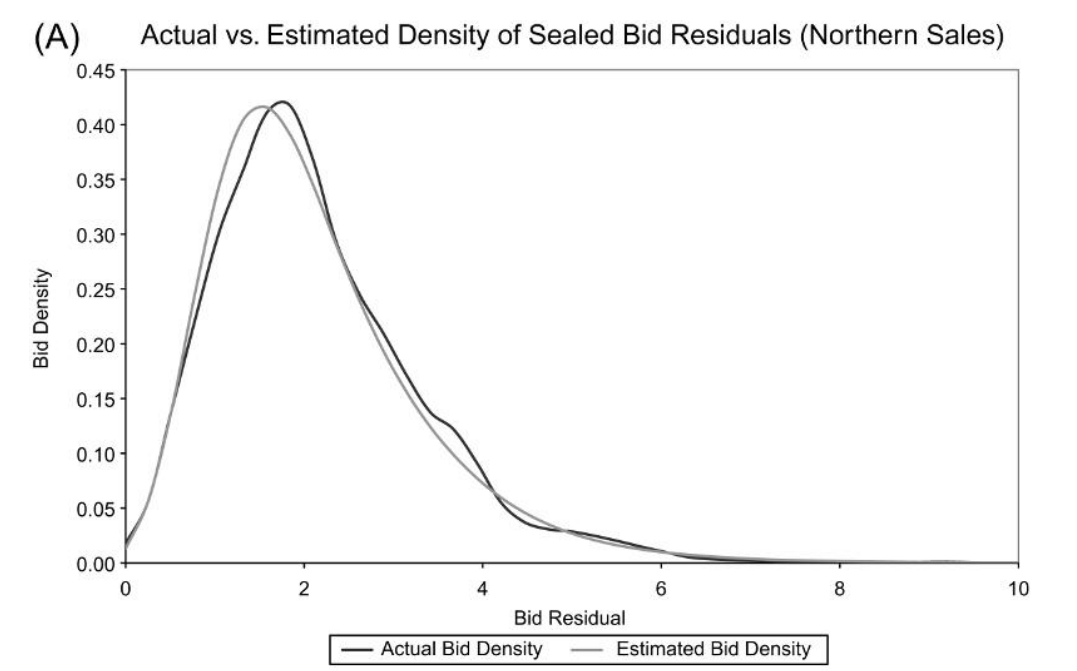
\includegraphics[width=0.49\textwidth]{figures/ch15/als2011_fig1a.png}\hfill
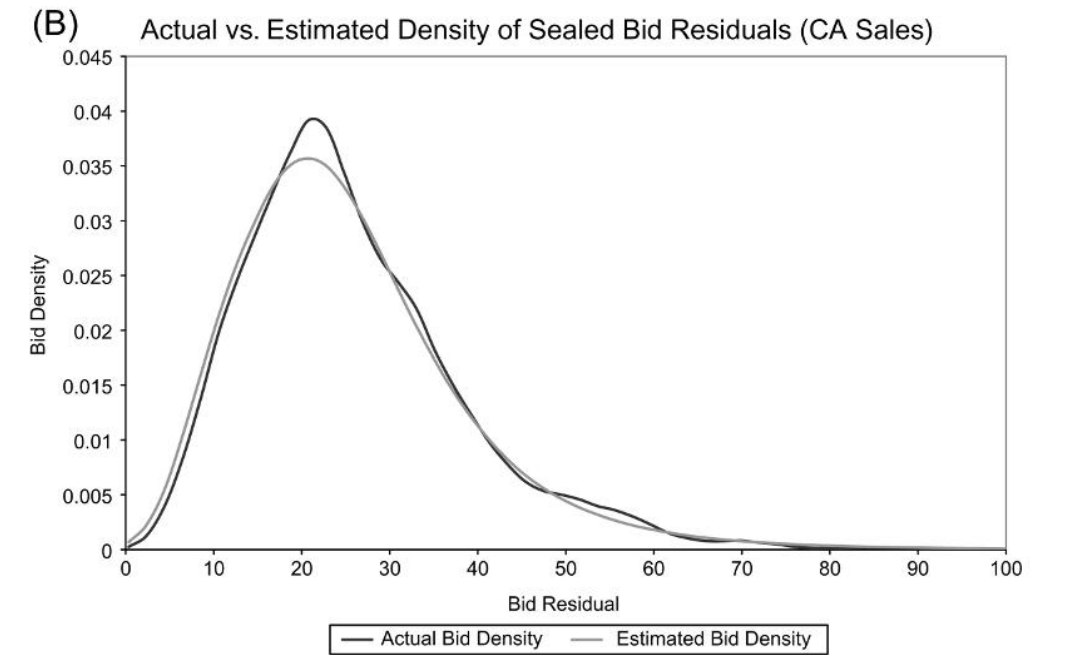
\includegraphics[width=0.49\textwidth]{figures/ch15/als2011_fig1b.png}
\caption{Actual (dark) and model-implied (light) densities of sealed-bid residuals, Northern sales (A)
and California sales (B). Residuals are bids divided by the fitted covariate index, and the actual density
is smoothed with a kernel. Source: \citet{AtheyLevinSeira2011}, Figure I.}
\label{fig:15-als-resid}
\end{figure}

\casehead{Recovering values}
Each sealed bid must be optimal against the rivals' bid distributions. Given $(Z,\omega,\bm N,\bm n)$, the
value behind a bid is given by \eqref{eq:15-als-inverse} \citep[eq.~(9)]{AtheyLevinSeira2011}. For the
Weibull distribution the reverse hazard rate has a closed form. Differentiating
\eqref{eq:15-als-weibull},
\[
g_k(b\mid\omega)=\omega\rho_kb^{\rho_k-1}\lambda_k^{-\rho_k}\exp\Bigl(-\omega\Bigl(\frac{b}{\lambda_k}\Bigr)^{\rho_k}\Bigr).
\]
Dividing by $G_k$ and multiplying numerator and denominator by $\exp(\omega(\frac{b}{\lambda_k})^{\rho_k})$,
\begin{equation}\label{eq:15-als-revhaz}
\frac{g_k(b\mid\omega)}{G_k(b\mid\omega)}=\frac{\omega\rho_kb^{\rho_k-1}\lambda_k^{-\rho_k}}{\exp\bigl(\omega(\frac{b}{\lambda_k})^{\rho_k}\bigr)-1}.
\end{equation}
Truncating the upper tail divides $g_k$ and $G_k$ by the same constant, so \eqref{eq:15-als-revhaz} is
unchanged below the truncation point. If $\omega$ were observed, each bid would map into a value, and the
value distributions would follow as in \cref{sec:15-gpv}. As \citet{Krasnokutskaya2011} observed, we can
still recover the value distributions for any value of $\omega$, because the bid functions are strictly
increasing \citep[eq.~(10)]{AtheyLevinSeira2011}:
\begin{equation}\label{eq:15-als-F}
F_k(v\mid Z,\omega,\bm N)=G_k\bigl(\xi_k^{-1}(v\mid Z,\omega,\bm N,\bm n)\bigm|Z,\omega,\bm N,\bm n\bigr).
\end{equation}

The parameterization implies a scaling property that ALS exploit \citep[p.~243]{AtheyLevinSeira2011}.
Write $s=\exp(Z\bm\theta^\lambda_Z+\bm N\bm\theta^\lambda_N)$, the part of the scale common to both
types, and $\lambda_k=s\tilde\lambda_k(\bm n)$. Then $G_k(b)=\tilde G_k(\frac{b}{s})$, where $\tilde G_k$ is
the distribution at $s=1$. Differentiating, $g_k(b)=\frac{1}{s}\tilde g_k(\frac{b}{s})$, so the reverse
hazard rates scale as $\frac{g_k}{G_k}(b)=\frac{1}{s}\frac{\tilde g_k}{\tilde G_k}(\frac{b}{s})$.
Substituting into \eqref{eq:15-als-inverse},
\[
\xi_i(b)=b+s\Biggl[\sum_{j\in\bm n\setminus i}\frac{\tilde g_j}{\tilde G_j}\Bigl(\frac{b}{s}\Bigr)\Biggr]^{-1}
=s\,\tilde\xi_i\Bigl(\frac{b}{s}\Bigr).
\]
Values, bids and therefore profits all scale with $s$. Profits need to be computed for a single value of
$(Z,\bm N)$ and then rescaled, which makes the many simulations below feasible.

A second property shows how the shape parameters govern market power.

\begin{proposition}[A floor on margins in the Weibull model]\label{prop:15-als-margin}
Under \eqref{eq:15-als-weibull}, for every bid $b>0$, every $\omega$ and every participant set,
\[
\frac{\xi_i(b)-b}{\xi_i(b)}\ \ge\ \frac{1}{1+\sum_{j\in\bm n\setminus i}\rho_j},
\]
with equality in the limit $b\to0$.
\end{proposition}

\begin{proof}
Let $x_j=\omega(\frac{b}{\lambda_j})^{\rho_j}>0$. By \eqref{eq:15-als-revhaz},
$\frac{g_j}{G_j}(b)=\frac{\rho_j}{b}\cdot\frac{x_j}{e^{x_j}-1}$. Since $e^{x}-1>x$ for $x>0$, each factor
$\frac{x_j}{e^{x_j}-1}$ lies in $(0,1)$ and tends to one as $x_j\to0$. Hence
$\sum_j\frac{g_j}{G_j}(b)<\frac{1}{b}\sum_j\rho_j$, and by \eqref{eq:15-als-inverse}
\[
\xi_i(b)-b>\frac{b}{\sum_j\rho_j},\qquad\text{so}\qquad\xi_i(b)>b\,\frac{1+\sum_j\rho_j}{\sum_j\rho_j}.
\]
Write $m=\xi_i(b)-b$. The margin $\frac{m}{b+m}$ increases in $m$, so it exceeds its value at
$m=\frac{b}{\sum_j\rho_j}$, which is $\frac{1}{1+\sum_j\rho_j}$. As $b\to0$, every $x_j\to0$ and the
inequality becomes an equality.
\end{proof}

The proposition is our derivation, not a result in ALS. It shows that the shapes, which measure how
concentrated bids are, discipline the markdowns. With the Northern estimates and two loggers and two mills,
$\rho_L=e^{1.134+2(0.016)+2(0.015)}=3.31$ and $\rho_M=3.56$. Every logger bid in that configuration then
carries a margin of at least $\frac{1}{1+3.31+2(3.56)}=0.088$ (our calculation). ALS estimate the median
profit margin across all bids, averaging over $\omega$, at 9.5 percent in the North and 10.0 percent in
California, similar for mills and loggers \citep[p.~243]{AtheyLevinSeira2011}. The paper does not state
the formula for its margin, so the comparison is only indicative. Margins of this size suggest that sealed
bidding is quite competitive.

\begin{figure}[htbp]
\centering
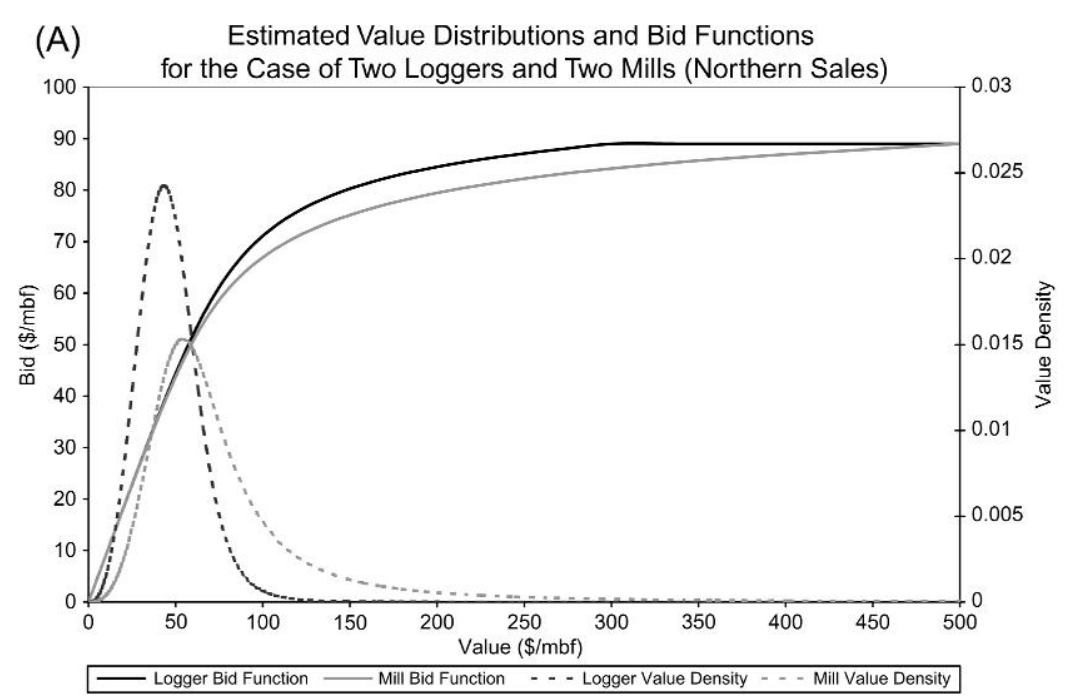
\includegraphics[width=0.49\textwidth]{figures/ch15/als2011_fig2a.png}\hfill
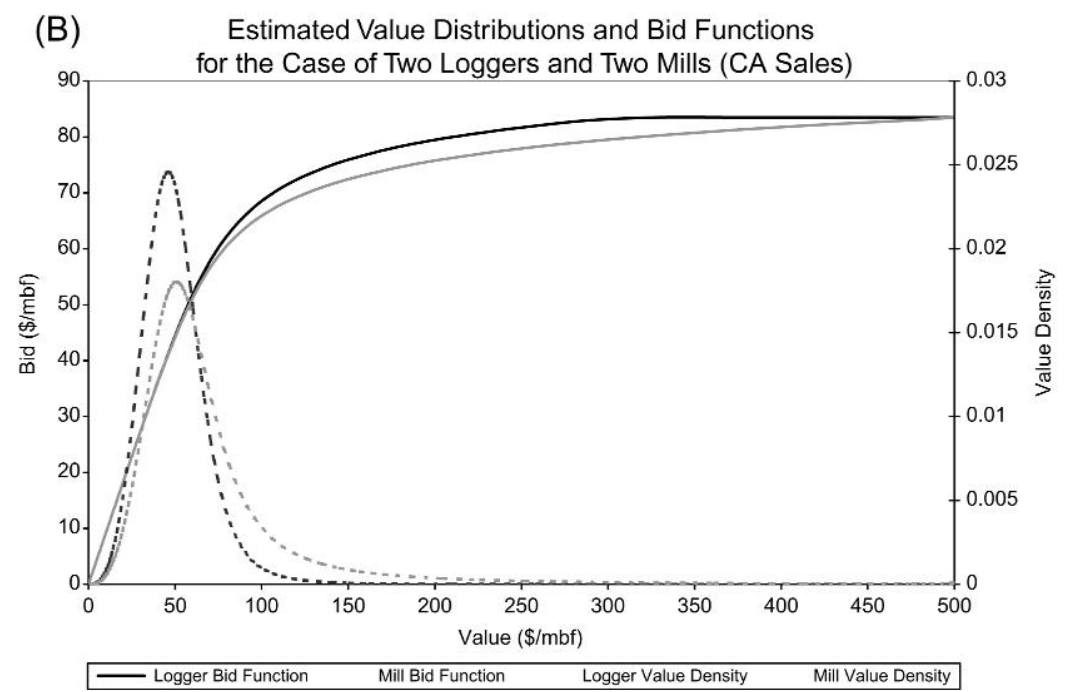
\includegraphics[width=0.49\textwidth]{figures/ch15/als2011_fig2b.png}
\caption{Estimated value densities (dashed, right axis) and equilibrium bid functions (solid, left axis)
for a sale with average covariates, $\omega=1$, two loggers and two mills, Northern sales (A) and California
sales (B). Dark curves are loggers and light curves are mills. The mill value density lies to the right,
and the mill bid function lies below the logger bid function. Source: \citet{AtheyLevinSeira2011},
Figure II.}
\label{fig:15-als-values}
\end{figure}

\Cref{fig:15-als-values} shows the recovered primitives for a sale with average covariates, $\omega=1$ and
two participants of each type. ALS compute the bid functions by inverting $\xi_k$ for the fitted bid
distributions. The mill value distribution is shifted well to the right of the logger distribution. The
mill bid function lies below the logger bid function, so mills bid less than loggers at any given value
(p.~243). This is property (i) of \cref{prop:14-maskin-riley}, the result of \citet{MaskinRiley2000}, now
found in estimated primitives.

\casehead{Checking uniqueness}
Prediction (P2) needs $\pi^{\mathrm s}_M(n_L,n_M+1)>\pi^{\mathrm s}_L(n_L,n_M)$. ALS compute the profits by
simulation \citep[pp.~243--245]{AtheyLevinSeira2011}.
\begin{enumerate}[label=(\arabic*)]
\item Draw $\omega$ from the estimated Gamma distribution.
\item For each participant, draw a bid from $\hat G_L(\cdot\mid\omega)$ or $\hat G_M(\cdot\mid\omega)$.
\item Convert each bid into a value with $\hat\xi_k$ from \eqref{eq:15-als-inverse} and \eqref{eq:15-als-revhaz}.
\item Identify the winner, the highest bidder, and record its profit $v-b$. Losers earn zero.
\item Repeat 5,000 times for each configuration with up to 8 mills and 25 loggers, and average.
\end{enumerate}
The inequality holds for all configurations and every tract in the sample (p.~245). By
\cref{prop:14-als-unique}, the estimated model has a unique type-symmetric entry equilibrium for every
tract, whatever the entry cost. In that equilibrium, if loggers enter with positive probability, every mill
enters.

\casehead{Entry costs}
ALS observe loggers entering 85 percent of Northern sales and 88 percent of California sales (p.~245).
Since potential exceeds actual logger entry almost everywhere, loggers must randomize, and a randomizing
logger is indifferent. For format $\tau$, \citep[eq.~(11)]{AtheyLevinSeira2011}
\begin{equation}\label{eq:15-als-indiff}
\Pi^\tau_L(Z,\bm N)=\sum_{n_L=1}^{N_L}\pi^\tau_L(Z,\bm N,\bm n)\,\Pr\bigl[\bm n\mid Z,\bm N,i\in\bm n,\tau\bigr]=K(Z,\bm N),
\end{equation}
with $n_M=N_M$. This is the general condition \eqref{eq:14-entry-indiff} and the identification argument of
\cref{prop:15-entry-ident}. Given that logger $i$ enters, each of the other $N_L-1$ potential loggers enters
independently with probability $p^\tau(Z,\bm N)$, so \citep[eq.~(12)]{AtheyLevinSeira2011}
\begin{equation}\label{eq:15-als-binom}
\Pr\bigl[n_L\mid Z,\bm N,i\in\bm n,\tau\bigr]=\binom{N_L-1}{n_L-1}p^\tau(Z,\bm N)^{n_L-1}\bigl(1-p^\tau(Z,\bm N)\bigr)^{N_L-n_L}.
\end{equation}
For sealed sales the entry probability is a logit \citep[eq.~(13)]{AtheyLevinSeira2011},
\begin{equation}\label{eq:15-als-logit}
p^{\mathrm s}(Z,\bm N)=\frac{\exp(Z\bm\gamma_Z+\bm N\bm\gamma_N)}{1+\exp(Z\bm\gamma_Z+\bm N\bm\gamma_N)},
\end{equation}
where ALS write $\alpha$ for $\bm\gamma$. In sale $t$ the number of entering loggers is binomial with
$N_{L,t}$ trials and success probability $p_t=p^{\mathrm s}(Z_t,\bm N_t)$. Up to a constant, the
log-likelihood is
\begin{equation}\label{eq:15-als-loglik}
\ln L(\bm\gamma)=\sum_{t\,\in\,\text{sealed}}\Bigl[n_{L,t}\ln p_t+\bigl(N_{L,t}-n_{L,t}\bigr)\ln(1-p_t)\Bigr].
\end{equation}
Let $\bm x_t=(Z_t,\bm N_t)$ be the row of regressors. For the logit, $\frac{\partial\ln p_t}{\partial\bm\gamma}=(1-p_t)\bm x_t^\T$ and
$\frac{\partial\ln(1-p_t)}{\partial\bm\gamma}=-p_t\bm x_t^\T$. The score is therefore
\[
\frac{\partial\ln L}{\partial\bm\gamma}=\sum_t\Bigl[n_{L,t}(1-p_t)-(N_{L,t}-n_{L,t})p_t\Bigr]\bm x_t^\T=\sum_t\bigl(n_{L,t}-N_{L,t}p_t\bigr)\bm x_t^\T .
\]
The maximum likelihood estimator sets the sum of observed minus expected entrants, weighted by the
covariates, to zero. The estimates are the entry columns of \cref{tab:15-als-estimates}.

The entry cost then follows without further estimation. ALS combine the simulated profits
$\hat\pi^{\mathrm s}_L(Z,\bm N,\bm n)$ with $\hat p^{\mathrm s}(Z,\bm N)$ in
\eqref{eq:15-als-indiff} and \eqref{eq:15-als-binom}, and set $\hat K(Z,\bm N)=\hat\Pi^{\mathrm s}_L(Z,\bm N)$ for each
tract. The median entry cost is \$2,870 (s.e.\ \$325) in the North and \$5,056 (s.e.\ \$673) in California
\citep[p.~246]{AtheyLevinSeira2011}. Cruising a tract can cost several thousand dollars, so these figures
are plausible. For comparison, the median expected profit of a mill in a sealed sale is roughly \$45,000
gross of entry costs (footnote 26). The median entry costs are thus about 6.4 and 11.2 percent of that
profit, the ratios reported by \citet[p.~91]{HortacsuPerrigne2021} (\cref{tab:15-entry-costs}). Two checks support the specification. If loggers entered with
probability zero in some tracts, the data would contain significantly more sales without logger entry than
the binomial model predicts, and they do not (footnote 25). Under pure-strategy entry, revealed preference
gives fairly tight bounds on entry costs that are similar to the point estimates (footnote 26).

\Cref{fig:15-als-entry} illustrates the logic and anticipates the open-auction prediction. The logger's
entry payoff falls with the probability that other loggers enter. A logger earns less in an open auction
for any participant set, so the open curve lies below the sealed curve. With the cost $K$ fixed, the
equilibrium entry probability is lower under open bidding.

\begin{figure}[htbp]
\centering
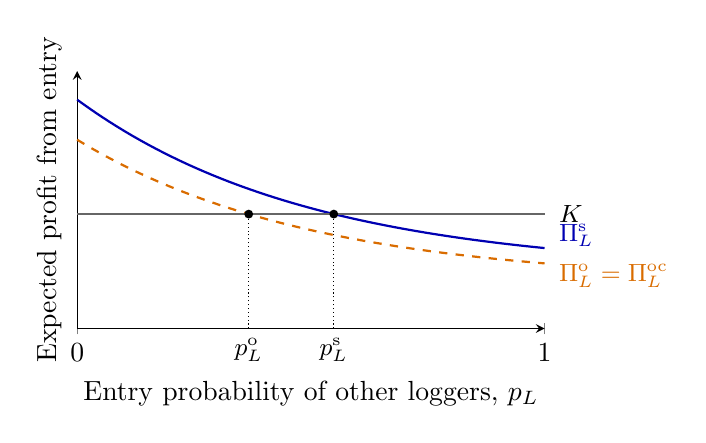
\begin{tikzpicture}
\begin{axis}[
  width=0.62\textwidth, height=0.40\textwidth,
  xmin=0, xmax=1, ymin=0, ymax=9,
  xlabel={Entry probability of other loggers, $p_L$},
  ylabel={Expected profit from entry},
  axis lines=left, xtick={0,1}, ytick=\empty,
  clip=false, every axis plot/.append style={thick}]
\addplot[domain=0:1, samples=60, blue!70!black] {2+6*exp(-2*x)};
\addplot[domain=0:1, samples=60, orange!85!black, dashed] {1.6+5*exp(-2*x)};
\addplot[domain=0:1, samples=2, black!60] {4};
\node[anchor=west, font=\small, blue!70!black] at (axis cs:1.01,3.25) {$\Pi^{\mathrm s}_L$};
\node[anchor=west, font=\small, orange!85!black] at (axis cs:1.01,1.85) {$\Pi^{\mathrm o}_L=\Pi^{\mathrm{oc}}_L$};
\node[anchor=west, font=\small] at (axis cs:1.01,4) {$K$};
\draw[densely dotted] (axis cs:0.549,0) -- (axis cs:0.549,4);
\draw[densely dotted] (axis cs:0.367,0) -- (axis cs:0.367,4);
\fill (axis cs:0.549,4) circle (1.6pt);
\fill (axis cs:0.367,4) circle (1.6pt);
\node[below, font=\small] at (axis cs:0.549,0) {$p^{\mathrm s}_L$};
\node[below, font=\small] at (axis cs:0.367,0) {$p^{\mathrm o}_L$};
\end{axis}
\end{tikzpicture}
\caption{Logger entry in the type-symmetric equilibrium with $p_M=1$ (schematic, not estimated). The
entry payoff of a logger falls in the entry probability of the other loggers. Indifference with the entry
cost $K$ pins down $p^{\mathrm s}_L$ in sealed auctions and the lower $p^{\mathrm o}_L$ in open auctions.
Mill collusion in open auctions leaves logger profits unchanged ($\Pi^{\mathrm{oc}}_L=\Pi^{\mathrm o}_L$),
so it leaves logger entry unchanged.}
\label{fig:15-als-entry}
\end{figure}

\subsection{Out-of-sample predictions and the competitiveness of open auctions}\label{sec:15-als-predict}

With the value distributions and entry costs in hand, ALS predict the outcome of every sale and compare
the predictions with the data \citep[pp.~247--248]{AtheyLevinSeira2011}. The procedure has four parts.
\begin{enumerate}[label=(\arabic*)]
\item \emph{Sealed sales.} The entry logit gives the distribution of entering loggers, and mill entry is
known. The fitted bid distributions, integrated over $\omega$, give bidding outcomes for each participant
set. Combining the two gives outcomes conditional on the tract characteristics alone.
\item \emph{Open sales, competitive.} For each simulated auction, draw $\omega$ and draw a value for each
participant from $\hat F_L(\cdot\mid Z,\omega,\bm N)$ or $\hat F_M(\cdot\mid Z,\omega,\bm N)$ via
\eqref{eq:15-als-F}. Then record the price $P^{\mathrm o}=\max\{V^{(n-1:n)},r\}$, the second-highest
participant value or the reserve price.
\item \emph{Open sales, collusive.} All participating mills except the one with the highest value drop out
at once. The price is the second-highest value in the set formed by the top mill and the loggers, or the
reserve price.
\item \emph{Open entry.} Mill entry equals the potential mill count. The logger entry probability
$p^{\mathrm o}_L$ is the unique solution of $\hat\Pi^{\mathrm o}_L(Z,\bm N;p_L)=\hat K(Z,\bm N)$. Uniqueness
holds because $\hat\Pi^{\mathrm o}_L$ falls monotonically in $p_L$ \citep[footnote 27]{AtheyLevinSeira2011}.
By prediction (P5), the same $p^{\mathrm o}_L$ applies under collusion.
\end{enumerate}
Standard errors come from a parametric bootstrap. ALS draw parameters from the estimated asymptotic
distribution of the \cref{tab:15-als-estimates} estimates and repeat the whole calculation for each draw
(p.~248). Column (2) of \cref{tab:15-als-predict} conditions on the observed participants, and column (3)
predicts entry as well.

\begin{table}[htbp]
\centering
\caption{Actual outcomes and outcomes predicted by the estimated model}
\label{tab:15-als-predict}
\small
\begin{tabular}{@{}lrccc@{}}
\toprule
 & $N$ & (1) Actual & (2) Predicted, & (3) Predicted,\\
 & & & bidding only & bidding and entry\\
\midrule
\multicolumn{5}{@{}l}{\textit{A. Northern sales}}\\
\multicolumn{5}{@{}l}{\quad Sealed-bid sales}\\
\quad Average bid & 1,492 & 59.6 & 58.2 (1.4) & 57.4 (1.3)\\
\quad Average logger bid & 1,096 & 50.8 & 48.7 (1.4) & 47.4 (1.4)\\
\quad Average mill bid & 396 & 83.8 & 84.7 (2.7) & 85.2 (2.7)\\
\quad Average sale price & 339 & 69.4 & 69.9 (1.4) & 70.4 (1.6)\\
\quad Average revenue (thousands) & 339 & 111.4 & 108.1 (4) & 109.9 (4.2)\\
\quad Percent of sales won by loggers & 339 & 68.1 & 68.0 (0.90) & 65.0 (0.01)\\
\quad Average logger entry & 339 & 3.23 & & 3.23 (0.09)\\
\multicolumn{5}{@{}l}{\quad Open auction sales}\\
\quad Average sale price, competition & 732 & 63.3 & 67.9 (1.8) & 67.8 (2.1)\\
\quad Average sale price, collusion & 732 & 63.3 & 44.2 (1.3) & 44.1 (2.2)\\
\quad Average revenue, competition & 732 & 144.7 & 152.7 (6.8) & 154.8 (7.9)\\
\quad Average revenue, collusion & 732 & 144.7 & 61.0 (2) & 64.7 (5.0)\\
\quad Percent of sales won by loggers & 732 & 59.0 & 56.0 (0.01) & 54.4 (0.02)\\
\quad Average logger entry & 732 & 2.75 & & 2.67 (0.17)\\[3pt]
\multicolumn{5}{@{}l}{\textit{B. California sales}}\\
\multicolumn{5}{@{}l}{\quad Sealed-bid sales}\\
\quad Average bid & 1,630 & 73.6 & 74.7 (2.3) & 74.2 (2.3)\\
\quad Average logger bid & 1,150 & 64.0 & 63.6 (2.1) & 62.3 (2.4)\\
\quad Average mill bid & 480 & 96.5 & 101.2 (3.5) & 102.8 (3.8)\\
\quad Average sale price & 382 & 80.4 & 83.8 (2.1) & 84.4 (2.4)\\
\quad Average revenue (thousands) & 382 & 103.1 & 110.7 (3.8) & 111.9 (4.0)\\
\quad Percent of sales won by loggers & 382 & 66.8 & 66.4 (1.2) & 62.6 (1.3)\\
\quad Average logger entry & 382 & 3.01 & & 3.01 (0.07)\\
\multicolumn{5}{@{}l}{\quad Open auction sales}\\
\quad Average sale price, competition & 325 & 85.1 & 87.2 (2.7) & 86.7 (3.1)\\
\quad Average sale price, collusion & 325 & 85.1 & 46.1 (1.2) & 51.0 (1.6)\\
\quad Average revenue, competition & 325 & 227.0 & 244.7 (9.7) & 242.4 (10.9)\\
\quad Average revenue, collusion & 325 & 227.0 & 93.2 (2.6) & 112.9 (5.6)\\
\quad Percent of sales won by loggers & 325 & 50.5 & 48.2 (1.1) & 43.6 (1.8)\\
\quad Average logger entry & 325 & 1.95 & & 1.90 (0.13)\\
\bottomrule
\end{tabular}

\smallskip
\begin{minipage}{\linewidth}
\footnotesize\textit{Notes.} Reproduced from \citet[Table V]{AtheyLevinSeira2011}. Bids and prices in 1982
dollars per mbf, revenue in thousands of 1982 dollars. Column (1) shows average outcomes. Column (2) shows
predictions for the same sales conditional on the observed entrants. Column (3) shows predictions of the
equilibrium model of entry and bidding. Parametric bootstrap standard errors in parentheses, as printed
(the paper prints a second standard error, 0.1, below the row for Northern sealed-bid logger entry). The
standard errors for the percent of sales won by loggers appear in mixed units in the original.
\end{minipage}
\end{table}

\casehead{In-sample fit}
The sealed-bid rows measure fit, since these sales were used in estimation. In the North the average sale
price is 69.4 dollars per mbf, against predictions of 69.9 with observed entry and 70.4 with predicted
entry \citep[p.~248]{AtheyLevinSeira2011}. Average logger and mill bids and the share of sales won by
loggers are also close. The largest discrepancy is in California, where the model overpredicts the sale
price, 84.4 or 83.8 against 80.4, and the revenue.

\casehead{Out-of-sample entry and allocation}
The open-auction rows are the demanding test. The model predicts open-auction logger entry of 2.67 in the
North against 2.75 observed, and 1.90 in California against 1.95 \citep[p.~250]{AtheyLevinSeira2011}. The
model therefore explains the entry gap between formats, one of the main departures from revenue
equivalence. It is less successful with allocation. It predicts that loggers win 54.4 percent of Northern
open sales, or 56.0 percent with observed entry, against 59.0 percent observed. California shows a similar
underprediction.

\casehead{Out-of-sample prices and conduct}
In California the competitive model predicts an open-auction price of 87.2 with observed entry and 86.7
with predicted entry, against 85.1 observed. The model reproduces the absence of a price difference between
formats. The North is different. The competitive model predicts 67.9 or 67.8, and the fully collusive model
44.2 or 44.1. The observed average is 63.3. Accounting for sampling error, ALS reject both models at
conventional levels. ``Mildly cooperative'' behavior by participating mills fits better than either extreme
(pp.~250--251). A linear interpolation between the competitive and collusive predictions in column (2)
gives a cooperation share of $\frac{67.9-63.3}{67.9-44.2}=0.19$ (our calculation). ALS use 18 percent as the
share that rationalizes Northern open prices in their welfare analysis.

Two robustness arguments strengthen the conclusion (p.~251). If sealed bidding were partly collusive, the
inferred values would be higher, and open prices would look even less competitive. ALS also examined the
open sales whose predicted price lies far above the actual price and found no obvious pattern.

\casehead{Where collusion should show up}
Statistical detection of collusion is hard \citep{BajariYe2003}, so ALS test a sharper implication of
(P5). With zero or one participating mill the competitive and collusive models predict the same price.
Any effect of mill collusion must appear in sales with two or more mills.
\Cref{tab:15-als-mills,fig:15-als-mills} split the Northern sales by mill participation.

\begin{table}[htbp]
\centering
\caption{Actual and predicted sale prices by mill participation, Northern sales}
\label{tab:15-als-mills}
\small
\begin{tabular}{@{}lrccc@{}}
\toprule
 & $N$ & (1) Actual & (2) Predicted, & (3) Predicted,\\
 & & & bidding only & bidding and entry\\
\midrule
\multicolumn{5}{@{}l}{\textit{Zero mills}}\\
\quad Sealed-bid sales & 181 & 51.7 & 51.4 & 51.4\\
\quad Open auction sales & 321 & 49.8 & 50.5 & 47.1\\
\multicolumn{5}{@{}l}{\textit{One mill}}\\
\quad Sealed-bid sales & 70 & 66.8 & 64.6 & 66.9\\
\quad Open auction sales & 150 & 50.0 & 52.2 & 59.5\\
\multicolumn{5}{@{}l}{\textit{Two or more mills}}\\
\quad Sealed-bid sales & 88 & 108.1 & 112.1 & 112.2\\
\quad Open auction sales & 261 & 87.5 & 98.5 & 98.0\\
\bottomrule
\end{tabular}

\smallskip
\begin{minipage}{0.84\linewidth}
\footnotesize\textit{Notes.} Reproduced from \citet[Table VI]{AtheyLevinSeira2011}. Average sale prices
in 1982 dollars per mbf. Predictions assume competitive bidding.
\end{minipage}
\end{table}

\begin{figure}[htbp]
\centering
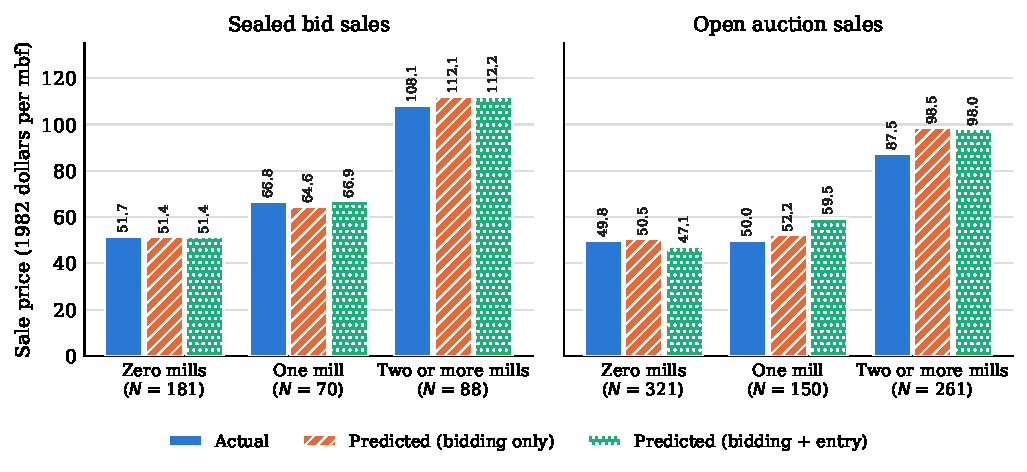
\includegraphics[width=0.92\textwidth]{figures/ch15/als_tableVI.pdf}
\caption{Actual and predicted competitive sale prices by mill participation, Northern sales. Drawn from
the numbers in \citet[Table VI]{AtheyLevinSeira2011}. With observed entry, the competitive model fits open prices
with zero or one mill and overpredicts them with two or more mills.}
\label{fig:15-als-mills}
\end{figure}

With exogenous entry, column (2), the competitive model predicts open prices accurately with zero mills
(50.5 against 49.8) and one mill (52.2 against 50.0). With two or more mills it predicts 98.5 against an
observed 87.5, a shortfall of 11 percent (our calculation), as the collusion theory implies
\citep[p.~252]{AtheyLevinSeira2011}. In sealed sales with two or more mills the shortfall is 4 percent.
Column (3) is less sharp, because the model does not fit realized logger entry cell by cell. For open sales
it predicts 3.31, 2.26 and 1.06 entering loggers in sales with zero, one and two or more mills, against
3.76, 3.32 and 1.77 observed (footnote 28). Column (2) uses observed entry and isolates the bidding margin.
Since the theory predicts identical entry under competition and collusion, that margin is where the two
hypotheses differ.

\subsection{Counterfactual comparison of formats}\label{sec:15-als-welfare}

ALS finally take the estimates as the true primitives and ask what would happen if every tract were sold by
one format \citep[Section V.C]{AtheyLevinSeira2011}. For each tract and format they compute expected entry,
the expected price and revenue, the probability that a logger wins and the expected surplus. Surplus is the
winner's value net of the entry costs sunk by all participants. Under exogenous entry, participation is
fixed at its realized value. Under endogenous entry, both formats are solved for their entry equilibria.
For open auctions they consider competitive mills and mills that cooperate 18 percent of the time.
\Cref{tab:15-als-welfare} reproduces the results.

\begin{table}[htbp]
\centering
\caption{Counterfactual outcomes of sealed and open auctions}
\label{tab:15-als-welfare}
\small
\setlength{\tabcolsep}{4.5pt}
\begin{tabular}{@{}lccccc@{}}
\toprule
 & (1) & (2) & (3) & (4) & (5)\\
 & Sealed & Open & Sealed $-$ open & Open & Sealed $-$ open\\
 & & (competitive) & (1) $-$ (2) & (partly collusive) & (1) $-$ (4)\\
\midrule
\multicolumn{6}{@{}l}{\textit{A. Northern sales ($N=1{,}071$)}}\\
\multicolumn{6}{@{}l}{\quad Exogenous entry}\\
\quad Average sale price & 68.56 & 68.53 & 0.03 (0.04) & 64.58 & 3.98 (0.24)\\
\quad Average revenue & 138.33 & 138.64 & $-0.32$ (0.06) & 124.33 & 14.00 (1.22)\\
\quad Average surplus & 176.99 & 177.06 & $-0.08$ (0.02) & & \\
\quad Percent won by loggers & 60.14 & 59.68 & 0.46 (0.16) & & \\
\multicolumn{6}{@{}l}{\quad Endogenous entry}\\
\quad Average sale price & 69.68 & 68.19 & 1.49 (0.71) & 64.11 & 5.57 (0.82)\\
\quad Average revenue & 143.04 & 139.87 & 3.17 (2.24) & 125.32 & 17.72 (2.74)\\
\quad Average surplus & 156.53 & 156.84 & $-0.30$ (2.70) & & \\
\quad Percent won by loggers & 59.65 & 57.19 & 2.46 (0.00) & & \\
\quad Logger entry & 3.10 & 2.76 & 0.34 (0.12) & & \\[3pt]
\multicolumn{6}{@{}l}{\textit{B. California sales ($N=707$)}}\\
\multicolumn{6}{@{}l}{\quad Exogenous entry}\\
\quad Average sale price & 85.53 & 85.20 & 0.32 (0.07) & 79.39 & 6.13 (0.39)\\
\quad Average revenue & 172.64 & 172.10 & 0.55 (0.13) & 154.43 & 18.21 (1.36)\\
\quad Average surplus & 203.61 & 203.65 & $-0.04$ (0.02) & & \\
\quad Percent won by loggers & 58.21 & 57.81 & 0.40 (0.002) & & \\
\multicolumn{6}{@{}l}{\quad Endogenous entry}\\
\quad Average sale price & 88.36 & 83.76 & 4.60 (2.26) & 78.55 & 9.81 (2.21)\\
\quad Average revenue & 182.38 & 168.20 & 14.18 (5.43) & 152.83 & 29.55 (5.39)\\
\quad Average surplus & 181.82 & 170.58 & 11.24 (6.86) & & \\
\quad Percent won by loggers & 55.84 & 52.66 & 3.18 (0.01) & & \\
\bottomrule
\end{tabular}

\smallskip
\begin{minipage}{\linewidth}
\footnotesize\textit{Notes.} Reproduced from \citet[Table VII]{AtheyLevinSeira2011}. Averages over all
tracts in a region of model predictions. Prices in 1982 dollars per mbf, revenue and surplus in thousands
of 1982 dollars. Exogenous entry uses the realized participants, and endogenous entry uses the equilibrium
entry model. The partly collusive open auction has mills cooperating 18 percent of the time. Bootstrap
standard errors in parentheses. The text of the paper (p.~253) states that with fixed participation sealed
bidding raises Northern revenue by \$320 per sale. The table prints a difference of $-0.32$ thousand,
consistent with its columns (1) and (2).
\end{minipage}
\end{table}

\casehead{A discrepancy in the source}
With fixed participation, the text of ALS reports a sealed-bid revenue gain of ``only \$320 per sale in
the Northern region and \$546 in California'' (p.~253).
Table VII prints a Northern difference of $-0.32$ thousand dollars. The table's own columns agree with the
negative sign, since $138.33-138.64=-0.31$. For California the text and table agree, $0.55$ thousand. We
report the table and conclude that with fixed participation the Northern revenue difference is a few
hundred dollars, of uncertain sign as printed.

\casehead{Lessons}
Four lessons emerge \citep[pp.~253--255]{AtheyLevinSeira2011}.
\begin{enumerate}[label=(\roman*)]
\item \emph{With fixed participation and competitive bidding, the format barely matters.} Revenue
differences are a few hundred dollars per sale, and the logger win probability changes by less than one
percentage point. The efficiency advantage of the open auction is under \$100 per sale in both regions.
The asymmetry between mills and loggers is substantial, yet its consequences for fixed participants are
small.
\item \emph{Entry magnifies the differences.} Both formats attract the same mills, but sealed bidding
attracts three to four more loggers per 10 sales (0.34 more per sale in the North). Loggers win 2 to 4
percentage points more sales. The sealed-bid revenue advantage rises to roughly \$3,000 per sale in the
North and \$14,000 in California, which is 2.3 and 8.4 percent of competitive open-auction revenue (our
calculation).
\item \emph{Efficiency comparisons are noisy.} The surplus difference stays small in the North. In
California the point estimate even favors sealed bidding, although sealed bidding is known to be less
efficient in equilibrium. The reason is that ALS estimate separate value distributions for each
participant configuration, and these estimates are not identical. Expectations over stochastic logger
entry weight the configurations differently across formats (footnote 29). Pooling the configurations would
break the link between the value distribution and the estimated bid distribution through the first-order
condition.
\item \emph{Collusion dominates.} Suppose mills cooperate 18 percent of the time in open auctions. Open bidding
then raises about \$14,000 less per Northern sale than competitive sealed bidding with fixed participation,
and over \$17,000 less with entry effects. The California differences are larger, \$18,210 and \$29,550 in
\cref{tab:15-als-welfare}.
\end{enumerate}
The revenue consequences of the format choice run mainly through the vulnerability of open auctions to
collusion. Gains from extra logger entry come second, and efficiency losses are small.

\subsection{Assessment}\label{sec:15-als-assessment}

\casehead{Contribution}
ALS combine three features that earlier work had treated separately: asymmetric bidders, unobserved
auction heterogeneity and endogenous participation \citep[p.~255]{AtheyLevinSeira2011}. Their entry model
recovers entry costs in dollars from post-entry profits and observed entry rates. Earlier entry models in
industrial organization infer profits relative to a normalized distribution of entry costs. Their main
methodological idea is to use variation in the rules for validation. The parameters come from one game and
are tested on another, which is a demanding out-of-sample check. The logic resembles the validation of
conduct estimates against direct cost data in \cref{ch:conduct}, with the second auction format in place of
the cost data. The approach also yields a conduct test. Behavior in the format least prone to collusion
serves as a benchmark for behavior in the format where collusion is suspected.

\casehead{Limitations}
Several assumptions deserve scrutiny.
\begin{itemize}
\item \emph{Functional form.} The Weibull and Gamma forms and the independence of $\omega$ from $Z$ are
maintained hypotheses. They pass an informal moment check and a formal specification test, but they drive
the extrapolation to open auctions. \citet{Roberts2013} argues that the reserve price itself carries
information about $\omega$ (\cref{sec:15-uh}). ALS include the reserve price in $Z$, so this would violate
the independence of $\omega$ and $Z$, and the large reserve-price coefficient in \cref{tab:15-als-estimates}
may partly proxy for $\omega$.
\item \emph{Competitive sealed bidding.} The benchmark assumes that sealed bidding is competitive. ALS
argue that sealed collusion would only strengthen the conclusion, but a cartel operating in both formats
would weaken the cross-format test.
\item \emph{Two types and a crude model of collusion.} Bidders are mills or loggers, and collusion is
modeled as perfect mill cooperation in a fraction of sales. Partial cooperation, cooperation that depends
on the identities of the mills, or coordinated entry would change the predictions.
\item \emph{Entry.} Point identification of entry costs relies on type-symmetric mixed strategies and on
the measured number of potential loggers, which contains error. Values learned only after entry rule out
selective entry.
\item \emph{Format selection.} In California the format varies strongly with size, and trimming keeps one
third of the sales. Selection on unobservables remains a concern there.
\item \emph{Open auctions as button auctions.} Open predictions assume that the price equals the
second-highest value. Jump bidding and bid increments break this equality (\cref{thm:15-ht}).
\item \emph{Two-step consistency.} Value distributions estimated separately by participant set need not
coincide, which produces the anomalous California surplus estimate.
\end{itemize}

\casehead{Follow-up work}
Later studies of Forest Service sales build on this model \citep[Section~2.6]{HortacsuPerrigne2021}.
\citet{AtheyCoeyLevin2013} evaluate small-business set-asides, sales reserved for firms with fewer than 500
employees. Their model keeps the entry and the mill-logger asymmetry of ALS and uses California's open and
sealed sales. Opening the set-aside sales to large firms would cut the share of sales won by small firms by
51 percent. It would raise revenue by 6 percent and surplus by 21 percent (pp.~98--99). A bid subsidy of
only 5 or 6 percent for small firms would keep their share of sales satisfactory. Prices would then rise by
4 percent and efficiency by 2 percent. \citet{RobertsSweeting2013} let bidders receive signals of their
values before entry, which makes entry selective. They compare the simultaneous open auction with a
sequential mechanism. In it, entrants arrive one at a time, observe the earlier offers and may jump bid to
deter later entry. With moderate selection and an entry cost of 2 percent of the average winning bid, the
sequential mechanism raises revenue by 1.8 percent. A simultaneous auction with an optimal reserve raises
it by 0.2 percent (pp.~99--100). \citet{Haile2001} studies resale. When winners can resell in a secondary
market, the values at which bidders drop out of an open auction rise with the number of bidders. Common
values predict the reverse, through the winner's curse. He instruments the number of bidders with the number
of sawmills in and near the county, and the evidence supports the model with resale (p.~100). The bounds of
\citet{AradillasLopezGandhiQuint2013} for correlated private values are applied to Oregon sales in
\cref{sec:15-reserve-asc}.

\section{Testing for Collusion with Auction Data}\label{sec:15-collusion}

Auction data seem ideal for detecting collusion. The rules are known, every bid and bidder is often
recorded, and the competitive benchmark is a fully specified game. Detection is nonetheless hard.
\citet{PorterZona1993}, in the working-paper version we follow, explain why.\footnote{We use NBER Working
Paper 4013 (March 1992) for the description of the tests. The published estimates are discussed in
\cref{sec:13-detection}.} Patterns often read as collusion can arise in competitive equilibria. Rotating
winners are consistent with competition when firms face capacity constraints. Comparisons of winning bids
with engineers' cost estimates can mislead, because the estimates may be inflated by past bids. Collusive
schemes take many forms \citep{HendricksPorter1989}. A cartel might rotate a single bid among its members,
or several members might submit higher \emph{complementary bids}, also called \emph{phantom bids}, to
create the appearance of competition. No single test can detect every scheme. A cartel that includes every
bidder could even choose complementary bids that pass any broadly applicable test. Its bids would mimic
competitive bids for some plausible realization of costs (Porter and Zona, working paper, pp.~2--3).

\citet[p.~211]{AtheyLevinSeira2011} sort the empirical approaches into three groups.
\Cref{tab:15-collusion-tests} summarizes them. The first group requires prior knowledge of the cartel's
existence and structure and compares suspected members with other bidders. The second derives in-sample
specification tests of the competitive model and treats collusion as the alternative. The third, which ALS
introduce, uses behavior under one format as the benchmark for another.

\begin{table}[htbp]
\centering
\caption{Approaches to detecting collusion with auction data}
\label{tab:15-collusion-tests}
\footnotesize
\begin{tabularx}{\linewidth}{@{}>{\raggedright\arraybackslash}p{2.3cm}>{\raggedright\arraybackslash}X>{\raggedright\arraybackslash}X>{\raggedright\arraybackslash}p{2.6cm}@{}}
\toprule
Approach & Maintained information & Implication tested & Examples\\
\midrule
Suspected members versus others & Identity of a candidate cartel, bid levels and ranks & Determinants of
non-winning cartel bids differ from those of the low cartel bid and of non-cartel bids & \citet{PorterZona1993,PorterZona1999}\\
\addlinespace
Specification tests of competition & Bidder and auction covariates & Conditional independence and
exchangeability of bids & \citet{BajariYe2003}\\
\addlinespace
Cross-format benchmark & A format presumed competitive & Prices in the suspect format fall short of
predictions only where theory says collusion bites & \citet{AtheyLevinSeira2011}\\
\addlinespace
Records of a known cartel & Knockout bids and side payments & Structural values and damages from the
cartel's internal bids & \citet{Asker2010}\\
\addlinespace
Super-plus factors & Bid histories, registrations, ownership after the sale & Transfers among bidders, no
rivalry within a subset, prompt resale, close losing bids & \citet{MarshallMarx2012}\\
\bottomrule
\end{tabularx}
\end{table}

\casehead{Porter and Zona: low cartel bids versus higher cartel bids}
Porter and Zona study state highway paving contracts on Long Island in the early 1980s. A set of five firms,
named in a bid-rigging conviction and related suits, forms a candidate cartel. Insiders described meetings
that designated a serious bidder and its bid, after which other members submitted higher bids. The cartel
did not rotate single bids. Several members bid on most jobs, which makes detection possible because ring
behavior can be compared with that of non-members. Each competitive bidder in a low-bid procurement auction
chooses its bid $b$ to maximize $(b-c_{it})\Psi_{it}(b)$, where $c_{it}$ is its cost on job $t$ and
$\Psi_{it}(b)$ its probability of submitting the lowest bid. The first-order condition is
\[
\Psi_{it}(b)+(b-c_{it})\Psi_{it}'(b)=0 ,
\]
the procurement analog of \eqref{eq:15-als-foc}. Costs are unobserved, so Porter and Zona approximate the
equilibrium bid by a log-linear rule,
\begin{equation}\label{eq:15-pz-bid}
\ln B_{it}=\alpha_t+W_{it}\bm\vartheta+\epsilon_{it},\qquad\E[\epsilon_{it}]=0,\qquad\Var(\epsilon_{it})=\sigma_t^2 .
\end{equation}
Here $\alpha_t$ is a job effect, $W_{it}$ are firm-job cost shifters such as capacity and backlog, and
$\epsilon_{it}$ is private cost information whose variance differs by job. Ordinary least squares on competitive bids
estimates $\bm\vartheta$, the job mean squared residual estimates $\sigma_t^2$, and feasible generalized
least squares reweights the data.

The sharper test uses the ranking of bids. Let $X_{it}=-\frac{W_{it}}{\hat\sigma_t}$ be the deflated cost
shifters with the sign reversed. If $-\epsilon_{it}$ is type I extreme value, the job effect cancels and the
probability that firm $i$ submits the lowest bid takes the logit form. The probability of the observed
ranking $b_{r_1t}<b_{r_2t}<\dots<b_{r_nt}$ is the rank-ordered logit
\begin{equation}\label{eq:15-pz-rank}
\Pr\bigl[b_{r_1t}<\dots<b_{r_nt}\bigr]=\prod_{m=1}^{n-1}\frac{\exp(\bm\vartheta X_{r_mt})}{\sum_{l=m}^{n}\exp(\bm\vartheta X_{r_lt})} .
\end{equation}
The likelihood factors into the probability of the lowest bid and the probabilities of the ranks above it.
Under correct specification and no phantom bidding, both parts carry the same coefficients. A likelihood
ratio test applied to competitive bids checks the specification. The same test applied to cartel bids
asks whether the low cartel bid and the higher cartel bids share determinants. Complementary bids are not
meant to win, so their ranking need not reflect cost differences. Porter and Zona find that ranks and
levels of non-cartel bids follow cost measures, while the ranks of higher cartel bids do not and differ
from those of the low cartel bid. A Chow test of a common bid equation for cartel and competitive firms, estimated as in their Table~4,
gives $F(76,319)=9.38$ (p.~33). For competitive bids, the likelihood ratio statistic for equal coefficients
across ranks is $4.30$ against a $\chi^2_6$ distribution, a $p$-value of $0.64$ (p.~33, estimates in Table~5).
For cartel bids it is $8.94$ against a $\chi^2_4$ distribution, a $p$-value of $0.063$ (p.~34, estimates in
Table~6). The $p$-values are our
computation. Page and table numbers refer to the NBER working-paper version of \citet{PorterZona1993}, and
\cref{sec:13-detection} reports the full estimates.

\casehead{Bajari and Ye: independence and exchangeability}
A second approach needs no list of suspects. In an independent private values model with symmetric
bidders, bids are independent across bidders conditional on the covariates, and the joint distribution of
bids is exchangeable \citep[Section 5.5]{AtheyHaile2007}. Suppose values have the form
$V_{it}=h(Z_{1t},Z_{2i},Z_{2(-i)},A_{it})$, where $Z_{1t}$ is an auction covariate, $Z_{2i}$ a bidder
covariate, $Z_{2(-i)}$ the rivals' covariates and $A_{it}$ an idiosyncratic factor with an exchangeable
distribution. Each bid then depends on $(Z_{1t},Z_{2i},Z_{2(-i)})$ and not on the bidder's identity. Two
regression tests follow. Residuals from regressions of bids on covariates should be uncorrelated across
bidders, and coefficients should be equal across bidders or classes of bidders.
\citet{BajariYe2003} apply both tests to highway construction procurement. Collusion is the alternative.
Rejection can also reflect omitted heterogeneity common to the bidders, the problem of \cref{sec:15-uh}.

\casehead{The structural signature}
ALS add a third approach with three steps. Estimate the model on the segment least prone to collusion,
sealed sales. Predict outcomes where collusion is suspected, open sales. Then look where theory says
collusion must appear, sales with two or more strong participants. The test exploits an implication of
theory that a cartel cannot easily mask: a ring of mills cannot lower prices in sales where at most one mill
participates. Its power comes from the structural model, which delivers the competitive benchmark for each
cell.

\casehead{Using a cartel's own records}
When records of a cartel's internal knockout auctions survive, the cartel's bids can be modeled directly.
\citet{Asker2010} uses such records for a ring of stamp dealers to estimate values, the ring's gains and the
harm to sellers and to non-members (\cref{sec:13-asker}).

\casehead{Theory and enforcement}
The theory of \cref{sec:14-collusion} explains why the format matters. In open and second-price auctions,
a ring in which the highest-value member bids and the others abstain is self-enforcing within the auction
(\cref{prop:14-robinson,prop:14-collusion-open}). In first-price auctions a ring needs the threat of future
punishment, the repeated-game enforcement of \cref{ch:collusion-theory}. Optimal collusion in repeated
first-price auctions with private information can take sophisticated forms. When the auctioneer reveals the
winning bid but not the winner's identity, optimal collusion has every member bid the reserve price with
equal chances of winning. \Citet[footnote 102]{AtheyHaile2007} summarize this result of
\citet{AtheyBagwellSanchirico2004}.

\citet[ch.~8]{MarshallMarx2012} compare what a ring gains under each format, with independent private
values and a fixed set of bidders. In an ascending auction the ring's highest-value member bids up to its
value and the other members never raise a hand (pp.~171--172). The ring gains only when it holds the two
highest values. It then wins at the highest value outside the ring instead of the second-highest value
overall. A bidder outside the ring who wins pays what it would have paid without the ring, so the ring
captures all of the gain (p.~176). In a first-price auction the ring's designated bidder faces fewer rivals
and lowers its bid. Bidders outside the ring respond by lowering their bids as well, and the equilibrium
is unique (pp.~174--175). The lower ring bid sometimes lets an outsider win when it would have lost under
competition. Part of the collusive gain then leaks to bidders outside the ring, so the incentive to collude
is typically weaker under sealed bidding (p.~176).

\begin{example}[Ring gains in an ascending auction]\label{ex:15-ring-gain}
Let $n=5$ bidders have values drawn independently from the uniform distribution on $[0,1]$, with no
reserve price, and let $k$ of them form a ring. The $m$-th lowest of five uniform values has mean
$\E[V^{(m:5)}]=\frac{m}{6}$. Let $J$ be the number of top values that the ring holds in an unbroken run
from the top. If $J\le1$, the price is the second-highest value overall. If $J=j\ge2$, the price is the
highest value outside the ring, $V^{(5-j:5)}$. Ring members are a random subset, so for $k=2$
\[
\Pr(J\le1)=1-\frac{2}{5}\cdot\frac{1}{4}=\frac{9}{10},\qquad \Pr(J=2)=\frac{2}{5}\cdot\frac{1}{4}=\frac{1}{10}.
\]
The expected price is
\[
\frac{9}{10}\cdot\frac{4}{6}+\frac{1}{10}\cdot\frac{3}{6}=0.600+0.050=0.650,
\]
against $\frac{4}{6}\approx0.667$ without the ring. The ring wins when it holds the top value, which
happens with probability $\frac{2}{5}$. Given that event, its member with the top value pays $\frac{4}{6}$
with probability $\frac{3}{4}$ and $\frac{3}{6}$ with probability $\frac{1}{4}$. The ring's expected
surplus is therefore
\[
\frac{2}{5}\Big[\frac{5}{6}-\Big(\frac{3}{4}\cdot\frac{4}{6}+\frac{1}{4}\cdot\frac{3}{6}\Big)\Big]
=\frac{2}{5}\cdot\frac{5}{24}=\frac{1}{12}\approx0.083 .
\]
Each member expects about $0.042$, against $\frac{1}{30}\approx0.033$ for a competitive bidder. Both numbers
match the first rows of \cref{tab:15-mm-rings}.
\end{example}

\begin{table}[htbp]
\centering
\caption{Ring size and auction format with five uniform bidders (Marshall and Marx 2012, Table 8.1)}
\label{tab:15-mm-rings}
{\small
\setlength{\tabcolsep}{4pt}
\begin{tabular}{ccccccc}
\toprule
 & \multicolumn{2}{c}{Expected price} & \multicolumn{2}{c}{Surplus per ring member} & \multicolumn{2}{c}{Surplus per outsider}\\
\cmidrule(lr){2-3}\cmidrule(lr){4-5}\cmidrule(lr){6-7}
Ring size $k$ & Ascending & First price & Ascending & First price & Ascending & First price\\
\midrule
1 & 0.667 & 0.667 & 0.033 & 0.033 & 0.033 & 0.033\\
2 & 0.650 & 0.651 & 0.042 & 0.035 & 0.033 & 0.037\\
3 & 0.600 & 0.609 & 0.056 & 0.041 & 0.033 & 0.049\\
4 & 0.467 & 0.506 & 0.083 & 0.057 & 0.033 & 0.086\\
5 & 0.000 & 0.000 & 0.167 & 0.167 & & \\
\bottomrule
\end{tabular}}

\smallskip
\begin{minipage}{0.93\textwidth}
\footnotesize \textit{Notes.} Values uniform on $[0,1]$, reserve price zero. Ascending entries and the
first-price entries for $k=1$ are analytic. The other first-price entries come from Monte Carlo simulation
with 100,000 draws, as reported by Marshall and Marx from earlier work of Marshall and coauthors.
\end{minipage}
\end{table}

\Cref{tab:15-mm-rings} shows both effects (pp.~181--182). A ring that does not include every bidder hurts the
seller more under ascending bidding, and its members gain more there. Outside bidders gain nothing from a
ring at an ascending auction, while at a first-price auction their surplus rises with the size of the ring.
The authors caution that this ranking is not a general result (p.~181, footnote 21, citing
\citealp{MaskinRiley2000}). Leakage also shapes who joins (Section 8.3, pp.~176--180). At an ascending
auction nothing leaks, so outsiders always want to join, and with symmetric bidders the ring wants everyone
in. At a sealed-bid auction a weak bidder may prefer to stay out and bid against a ring whose depressed bids
it can exploit. Membership also raises a sequencing problem (Section 8.3.2, pp.~179--180). The last bidder
to join adds a large gain, because its entry removes all remaining competition. If that bidder were paid its
contribution, every member would want to join last. Rings therefore fix the division of the gain before the
auction, with equal shares for symmetric members and the average of each member's marginal contributions
for asymmetric ones. Settling the split in advance also rules out conflicting claims and costly rent
seeking after the auction (p.~180).

\casehead{Auction design against rings}
\citet[ch.~10]{MarshallMarx2012} turn the comparison into design advice. Transparency helps a ring monitor
its members (pp.~200--202). Rules written to curb favoritism by public officials announce the set of
bidders before the sale and publish bids and identities after it, which serves rings as well. In early
spectrum auctions of the Federal Communications Commission, bidders chose their increments and used the last
three digits of their bids to signal to one another. Later designs fixed the increments and hid rivals'
identities until the auction closed. A right of last refusal for an incumbent supplier lets the incumbent
watch rivals' bids in real time, which deters deviations from a collusive agreement. Bidding under
disguised identities, or shill bids, makes deviations harder for a ring to police, especially at sealed-bid
auctions (pp.~202--205). With transparent registration a ring can suppress competition at an ascending
auction. It does so with a scheme in which the winning member pays the ring the excess of the
second-highest member report over the price. If identities are hidden during the bidding and registration
is not transparent, payments from winning members alone cannot suppress all competition. Information about
the object also matters. If bidders have more expertise than the seller, competitive bidding transfers the
rents from that expertise to the seller, which gives bidders an extra reason to collude. The frequency of
sales matters as well (p.~206). Regular, frequent sales make bid rotation and punishment easier, so an
auctioneer worried about collusion may hold fewer sales of larger lots at irregular intervals. Finally,
sealed bids leave a paper trail of losing bids, while ascending auctions often leave no record of who would
have bid (pp.~206--207). The authors list six measures (p.~207). Use sealed instead of ascending bids. Limit
information about rivals, outcomes and bids. Avoid rights of last refusal for incumbents. Allow multiple bids,
some under disguised identities. Choose disclosure of the seller's information with collusion in mind. Hold
auctions at long, irregular intervals. The first measure is the choice that Pinchot made for the Forest
Service (\cref{sec:15-als-question}).

\casehead{Plus factors for rings}
A \emph{plus factor} is evidence, beyond parallel prices, that supports an inference of collusion.
\citet[ch.~12]{MarshallMarx2012} focus on \emph{super-plus factors}, patterns whose probability without a
ring is close to zero (pp.~243--244). They stress those that a ring could not remove without changing how it
works. Two apply to both formats. The first is transfers among bidders, such as cash settlements
of a knockout or subcontracting and joint ownership arrangements that were not declared before the sale. The
second is a divergence between observed prices and the prices predicted by a model estimated on a
benchmark in which no ring is presumed to operate. This is the logic of the cross-format test of
\citet{AtheyLevinSeira2011}, with sealed sales as the benchmark and open sales as the suspect segment.

At an ascending auction the ring's rule is simple: members do not bid while another member is active
(pp.~244--246). The winner and the last underbidder, and any two bidders who compete directly, are then
never both members. A subset of bidders who never bid against each other at meaningful prices is therefore
a super-plus factor, although it may take many auctions to detect. Ascending auctions allocate efficiently,
so a prompt resale to another bidder who was present suggests a post-auction knockout. Light attendance is
not a super-plus factor, since rings may require members to attend. At a sealed-bid auction resale is
weaker evidence, because asymmetric bidders can produce inefficient allocations that resale corrects
(pp.~246--247). Nonwinning bids unrelated to values, the evidence that \citet{PorterZona1993} use, are not
substantive either, because a ring can rescale its losing bids freely. Close pairs of bids are more telling.
Suppose the top member has value \$100,000 and would bid \$90,000 under competition, but the ring wants it to
bid \$50,000. A member with value \$60,000 that expects less than \$10,000 from the ring would then gain by
bidding \$50,001 through a shill. To deter this, the ring has its top member bid more, say \$65,000, and has
another member bid just below. The frequent closeness of two bids then reveals the ring. A sudden switch
from ascending to sealed bidding is informative too (p.~248). A large price increase after the switch
suggests that a ring operated at the ascending auctions. No change is not evidence of no ring, and risk
aversion raises sealed-bid prices only modestly.

\casehead{Shill bidding in Russian oil and gas auctions}
The appendix to their chapter~12 studies ascending auctions for Russian oil and gas leases, which proceed
only if at least two bidders register (pp.~248--255). The government sets a reserve price and the
increments, and the lowest feasible bid is one increment above the reserve. The data cover 620 auctions
from 2004 to 2007. They are complete for 121 auctions and partial for 499. The complete auctions are larger,
with an average reserve of 71,503,769 rubles against 49,484,900. Five were canceled and one was awarded on
criteria other than price, which leaves 115. \Cref{tab:15-mm-russia} reproduces the distribution of winning
bids. Auctions with six or more participants always end at least 20 increments above the reserve. In 34
of the 43 two-bidder auctions, 79 percent, the winning bid is one or two increments above the reserve.
These 34 auctions have an average reserve of 27,515,294 rubles, less than half the average for all 620.

\begin{table}[htbp]
\centering
\caption{Winning bids in increments above the reserve, by number of participants (Marshall and Marx 2012,
Table 12.2)}
\label{tab:15-mm-russia}
\begin{tabular}{lcccccc}
\toprule
 & \multicolumn{5}{c}{Increments of the winning bid above the reserve} & \\
\cmidrule(lr){2-6}
Participants & 1 & 2 & 3--19 & 20--99 & 100 or more & Auctions\\
\midrule
2 & 53\% & 26\% & 9\% & 7\% & 5\% & 43\\
3 & 3\% & 9\% & 26\% & 41\% & 21\% & 34\\
4 & 8\% & 0\% & 15\% & 15\% & 62\% & 13\\
5 & 10\% & 10\% & 20\% & 10\% & 50\% & 10\\
6 or more & 0\% & 0\% & 0\% & 33\% & 67\% & 15\\
\addlinespace
Combined & 23\% & 13\% & 15\% & 22\% & 28\% & 115\\
\bottomrule
\end{tabular}

\smallskip
\begin{minipage}{0.93\textwidth}
\footnotesize \textit{Notes.} Subsample of 115 auctions with complete data, 2004--2007. Each row sums to 100
percent. Their Table 12.1 gives the same data as shares of all 115 auctions.
\end{minipage}
\end{table}

The identities point to shills (Table 12.3, pp.~251--253). The 34 auctions have 24 distinct winners, 26
distinct losers and 26 distinct ordered pairs. One bidder won six such auctions, always against the same
opponent, which never won any of the 620 auctions. The authors classify 13 losing bidders as \emph{pure
shills}. Each bid at most once, never won a lease in the 620 auctions, and never took part in an auction
without its winning partner. Two losers form a rotating pair, each winning against the other at one or two
increments, and the remaining 11 are occasional shills. The registration rule explains the pattern. A
license of interest to a single firm cannot be sold unless a second bidder registers, so the firm has an
incentive to bring one along. The authors note that their own static model of semitransparent auctions
leaves no role for shills in a well-functioning ring. Two pure shills did appear with their partners in
auctions with more than two bidders, which suggests dynamic motives or a strategic auctioneer.

\casehead{Evidence from timber sales}
Forest Service timber sales have produced several studies of collusion
\citep[Section~2.5]{HortacsuPerrigne2021}. Collusion was suspected in the 1970s and led to a congressional
hearing in 1977, but few cases were prosecuted (p.~96). \citet{BaldwinMarshallRichard1997} study Forest
Service oral auctions. They compare order-statistic models of competitive and cooperative bidding, in which a
winning ring member pays the highest value outside the ring. The supply of timber varied across years, and
oversupply alone could depress bids. After controlling for supply conditions, collusion explains the low bids
better (pp.~96--97). In British Columbia, sales are by first-price sealed bid. \citet{ListMillimetPrice2007}
treat collusion as an unobserved treatment and test conditional independence and exchangeability of bids, in
the spirit of \citet{BajariYe2003}. They flag 130 suspect bidders, and the evidence of collusion is mixed
(p.~97). \citet{Price2008} studies the spatial proximity of bidders. Firms located in the same town or nearby
bid 10 to 13 percent less, and exchangeability is rejected for firms in close proximity. Industry interviews
suggest that distance does not create asymmetry in values. With the same data, \citet{Schurter2020} shows that
an asymmetric independent private values model with collusion is not identified when the colluders are
unknown (pp.~97--98). An instrument that shifts competition but is independent of values given the reserve
price restores identification. His test asks, bidder by bidder, whether estimated values are independent of
the reserve. Seven firms fail it, and four of them do not bid competitively. Competitive bidding by these four
firms would raise revenue by 3.2 percent, a moderate cost of collusion.

\section{Divisible-Good Auctions: Bidding with Demand Schedules}\label{sec:15-divisible}

Treasury bills, central bank loans and electricity are sold in auctions in which each bidder states a
quantity for every price. The good is \emph{divisible}, so any share of the supply can be allocated. Such
auctions are also called \emph{share auctions}, after the model of \citet{Wilson1979}. Each bid is a demand
schedule, and the seller adds the schedules up to clear the market. This section gives a short treatment of
the format. Its message is that the logic of \cref{sec:15-gpv} carries over. The distribution of the
market-clearing price, given a bidder's own schedule, takes the place of the distribution of rival bids. We
set up the model, derive the first-order conditions under uniform and discriminatory pricing, and study one
application of each.

\subsection{The share auction with step bids}\label{sec:15-div-model}

A perfectly divisible good is sold to $N$ bidders. Quantities are measured as shares of the announced
supply. The quantity sold, $Q$, may be random, because the seller can adjust it after seeing the
bids. Its distribution is common knowledge. Bidder $i$ observes a private signal $s_i$, and signals are
independent across bidders. Winning the share $q$ gives the bidder the gross utility
\begin{equation}\label{eq:15-div-V}
V(q,s_i)=\int_0^q v(u,s_i)\,du ,
\end{equation}
where the \emph{marginal value} $v(q,s_i)$ is weakly decreasing in $q$ and strictly increasing in $s_i$.
Values are private, so $v$ does not depend on rivals' signals \citep[p.~978 and Assumptions~2 and 6]{Kastl2011}.

A bid is a \emph{step function}. Bidder $i$ submits $K_i$ \emph{bidpoints} $(b_k,q_k)$, $k=1,\dots,K_i$,
with prices $b_1>b_2>\dots>b_{K_i}$ and cumulative quantities $q_1<q_2<\dots<q_{K_i}$. The bidder demands
nothing at prices above $b_1$ and demands $q_k$ at prices in $(b_{k+1},b_k]$, with the convention
$b_{K_i+1}=0$ and $q_0=0$. The seller caps the number of bidpoints at $\bar K$, which is 10 in both
applications below. Bidders use far fewer steps than the cap allows, so the steps are a feature of the data
that a model must explain.

Let $y_j(p)$ be bidder $j$'s demand at price $p$. The \emph{residual supply} facing bidder $i$ is the
quantity left for it after its rivals' demands are met,
\begin{equation}\label{eq:15-div-rs}
RS_i(p)=Q-\sum_{j\neq i}y_j(p).
\end{equation}
It rises with $p$. It is random from $i$'s point of view, because it depends on rivals' signals and on $Q$.
The \emph{market-clearing price} $P^{\mathrm c}$ is the highest price at which total demand weakly exceeds
supply. Bids above $P^{\mathrm c}$ are filled in full. Demands exactly at $P^{\mathrm c}$ are scaled down in
proportion until the supply is exhausted, a rule called \emph{pro rata rationing on the margin}. Two payment
rules are common. Under \emph{uniform pricing} every unit won pays $P^{\mathrm c}$. Under
\emph{discriminatory pricing}, also called pay-as-bid, each unit won pays the bid on that unit. A bidder then
pays the area under its own step function up to the quantity it wins.

With continuous and strictly decreasing bid functions, as in \citet{Wilson1979}, residual supply crosses each
demand curve at a single point and nobody is rationed. With steps, residual supply is itself a step function.
It can cross bidder $i$'s schedule in two ways. On a vertical segment, $i$ receives exactly $q_k$ at a price
strictly between $b_{k+1}$ and $b_k$. On a horizontal segment, the price equals one of $i$'s bids and $i$ is
rationed. With private values and a continuous price grid, ties with positive probability are incompatible
with equilibrium, except possibly at bids above the bidder's marginal value \citep[p.~984 and
Appendix~B]{Kastl2011}. A bidder that expected a tie at a bid below its marginal value would gain by raising
that bid slightly. A rationed bidder is then the only marginal bidder, and it
receives the residual supply at its own bid.

\subsection{Uniform pricing: Kastl (2011)}\label{sec:15-kastl}

\casehead{Question} Economists agree that governments should sell their securities by auction, but they
disagree about the format. In a survey that \citet{Kastl2011} cites, 39 of 42 countries used discriminatory
pricing and only 3 used uniform pricing (p.~974). Theory does not rank the two formats on revenue or on
efficiency \citep[Section~10]{AtheyHaile2007}. Kastl asks how to measure the performance of a uniform-price
auction from bids when bidders submit only a few steps. His answer starts from the observation that steps
change the first-order conditions, and with them the values that bids reveal.

\casehead{The step first-order condition} Fix bidder $i$ with signal $s_i$, its bid $\{(b_k,q_k)\}$ and its
rivals' strategies. All probabilities and expectations below are over rivals' signals and the supply, given
$s_i$ and $i$'s bid. Write $A_k$ for the event $b_k>P^{\mathrm c}>b_{k+1}$, in which residual supply crosses
the vertical segment of $i$'s schedule at $q_k$.

\begin{proposition}[Step condition under uniform pricing]\label{prop:15-kastl}
Assume private values and pro rata rationing on the margin. In any Bayesian Nash equilibrium, for almost
every $s_i$, every step $k$ at which a tie has probability zero satisfies
\begin{equation}\label{eq:15-kastl-foc}
\Pr(A_k)\bigl[v(q_k,s_i)-\E(P^{\mathrm c}\mid A_k)\bigr]
=q_k\,\frac{\partial\,\E\bigl[P^{\mathrm c}\,\indic\{b_k\ge P^{\mathrm c}\ge b_{k+1}\}\bigr]}{\partial q_k} .
\end{equation}
Equivalently,
\begin{equation}\label{eq:15-kastl-mcmr}
v(q_k,s_i)=\E(P^{\mathrm c}\mid A_k)
+\frac{q_k}{\Pr(A_k)}\,\frac{\partial\,\E\bigl[P^{\mathrm c}\,\indic\{b_k\ge P^{\mathrm c}\ge b_{k+1}\}\bigr]}{\partial q_k} .
\end{equation}
\end{proposition}

\begin{proof}[Derivation]
We give the argument for a step at which ties have probability zero, as they do when $b_k<v(q_k,s_i)$. Fix a realization of rivals' signals and of the supply. Let $P(q)$ be the
inverse residual supply, the price at which $RS_i$ equals $q$. Three events involve step $k$.
\begin{enumerate}[label=(\roman*)]
\item On $A_k$, $b_{k+1}<P(q_k)<b_k$. Bidder $i$ wins $q_k$ at the price $P(q_k)$, and its payoff is
$V(q_k,s_i)-P(q_k)\,q_k$.
\item On $B_k$, $q_{k-1}<RS_i(b_k)<q_k$. The price is $b_k$, and $i$ is rationed to $RS_i(b_k)$.
\item On $B_{k+1}$, $q_k<RS_i(b_{k+1})<q_{k+1}$. The price is $b_{k+1}$, and $i$ is rationed to
$RS_i(b_{k+1})$.
\end{enumerate}
Raise $q_k$ slightly and hold the other bidpoints fixed. On $B_k$ and $B_{k+1}$ the payoff does not depend
on $q_k$, because $i$ receives the residual supply. Only the boundaries of the three events move. On the
boundary between $A_k$ and $B_k$ we have $P(q_k)=b_k$ and $RS_i(b_k)=q_k$, so the payoffs in (i) and (ii)
coincide. The same holds on the boundary between $A_k$ and $B_{k+1}$. Moving a boundary therefore has no
first-order effect, and only the change inside $A_k$ remains. Differentiating the payoff in (i) gives
\[
\frac{\partial\,\E[\text{payoff}]}{\partial q_k}
=\E\Bigl[\Bigl(v(q_k,s_i)-P(q_k)-q_k\,\frac{\partial P(q_k)}{\partial q_k}\Bigr)\indic\{A_k\}\Bigr].
\]
Set the derivative to zero and use $\E\bigl[P(q_k)\indic\{A_k\}\bigr]=\Pr(A_k)\,\E(P^{\mathrm c}\mid A_k)$:
\[
\Pr(A_k)\bigl[v(q_k,s_i)-\E(P^{\mathrm c}\mid A_k)\bigr]
=q_k\,\E\Bigl[\frac{\partial P(q_k)}{\partial q_k}\,\indic\{A_k\}\Bigr].
\]
It remains to rewrite the right side. The event $b_k\ge P^{\mathrm c}\ge b_{k+1}$ is the union of $A_k$,
$B_k$ and $B_{k+1}$. This union does not move with $q_k$, since a change in $q_k$ only shifts states among the
three events. Inside the union, $P^{\mathrm c}$ equals $P(q_k)$ on $A_k$ and the constants $b_k$ and $b_{k+1}$
on the other two events. It is continuous across their boundaries. Hence
\[
\frac{\partial\,\E\bigl[P^{\mathrm c}\,\indic\{b_k\ge P^{\mathrm c}\ge b_{k+1}\}\bigr]}{\partial q_k}
=\E\Bigl[\frac{\partial P(q_k)}{\partial q_k}\,\indic\{A_k\}\Bigr] .
\]
Substituting gives \eqref{eq:15-kastl-foc}, and dividing by $\Pr(A_k)$ gives \eqref{eq:15-kastl-mcmr}. The
regularity needed to differentiate under the expectation is established in Lemmas~A2 to A4 of the appendix
of \citet{Kastl2011}.
\end{proof}

At a step with $b_k\ge v(q_k,s_i)$ a tie can have positive probability, and the condition gains two terms that
involve the rationed quantity (Kastl's eq.~(2)). Kastl uses \eqref{eq:15-kastl-mcmr} at every step. From discussions
with market participants, he argues that bidders ignore the effect of their demand on the rationed quantity.
An alternative estimator that allows for ties gives qualitatively similar, somewhat larger estimates with
large standard errors (Section~4.1 and Appendix~B.1).

\casehead{Interpretation} The left side of \eqref{eq:15-kastl-mcmr} is the value of the marginal unit. The
right side is its expected marginal expenditure. It adds the expected price on the vertical segment and the
expected rise in the clearing price on the $q_k$ units already bought. The bidder is a buyer facing a random,
upward-sloping residual supply curve, so the condition equates marginal value with marginal expenditure.
Kastl reads it as marginal cost equal to marginal revenue for an oligopolist facing uncertain demand. The
analogy extends the one of \cref{sec:14-proc-lerner}. There a single-object bidder chose a price, and the win
probability played the role of quantity. Here the bidder chooses quantities directly, and residual supply
plays the role of the demand curve. The second term on the right measures \emph{quantity shading}. The
bidder asks for less than the quantity at which its marginal value equals the expected price, because more
demand raises the price on all of its units.

\casehead{Steps versus smooth schedules} In Wilson's model with smooth schedules, the analog of
\eqref{eq:15-kastl-mcmr} holds at every price on the schedule (Kastl's eq.~(1)):
\begin{equation}\label{eq:15-wilson-uniform}
v\bigl(y(p),s_i\bigr)=p-y(p)\,\frac{H_x\bigl(p,y(p)\bigr)}{H_p\bigl(p,y(p)\bigr)},
\qquad H(p,x)=\Pr\bigl(x\le RS_i(p)\bigr).
\end{equation}
Here $H(p,x)$ is the probability that the clearing price is at most $p$ when $i$ demands $x$ at $p$, and
subscripts denote partial derivatives. Since $H$ falls in $x$ and rises in $p$, the markdown is nonnegative.
Every bid then lies weakly below the marginal value. The step condition differs in one place. Its reference
point is the expected clearing price on the segment, $\E(P^{\mathrm c}\mid A_k)$, which lies below the bid
$b_k$. Nothing in \eqref{eq:15-kastl-mcmr} therefore forces $b_k$ below $v(q_k,s_i)$.

\begin{corollary}[Bids above marginal values]\label{cor:15-kastl-above}
Under uniform pricing with step bids, a bidder may optimally bid above its marginal value
\citep[Corollary~1]{Kastl2011}.
\end{corollary}

\begin{proof}
Consider a bidder so small that its bid does not affect the distribution of $P^{\mathrm c}$, which is
continuous, and let $K_i=1$. Ties then have probability zero, and the right side of \eqref{eq:15-kastl-foc}
is zero. With $b_2=0$ the condition becomes
\[
v(q_1,s_i)=\E\bigl(P^{\mathrm c}\mid P^{\mathrm c}<b_1\bigr).
\]
Whenever $P^{\mathrm c}$ falls below $b_1$ with positive probability, the conditional mean lies strictly
below $b_1$. Hence $b_1>v(q_1,s_i)$.
\end{proof}

The intuition is that one step must serve every price below $b_1$. The bidder buys $q_1$ whenever the price
falls below $b_1$, so it equates the marginal value of the last unit with the average price at which that
unit is bought. The bid itself only decides whether the bidder buys at all. Exercise~\ref{exc:15-divisible}
shows that it equals the average value of the block, $\frac{V(q_1,s_i)}{q_1}$, which exceeds the marginal
value of the last unit.

The corollary matters for counterfactuals. Solving for an equilibrium under another format is hard, so
researchers often compare realized revenue with the revenue under \emph{truthful bidding}, in which every
bidder bids its marginal value schedule. With smooth schedules no bid exceeds value, so this revenue bounds
uniform-price revenue from above. \citet[Section~10]{AtheyHaile2007} describe how the working-paper version
of \citet{HortacsuMcAdams2010} used such a bound for Turkish treasury auctions. With steps the bound fails,
because bids can exceed values. Ignoring the steps also overstates values, since the smooth model adds the
shading term to the bid instead of to $\E(P^{\mathrm c}\mid A_k)$. Kastl argues that both errors bias
comparisons toward the discriminatory format (Sections~5.2.3 and 5.2.4).

\casehead{Identification and estimation} The bids are observed. Every unknown on the right of
\eqref{eq:15-kastl-mcmr} is therefore a functional of the distribution of $P^{\mathrm c}$ given $i$'s bid.
That distribution depends on the joint distribution of rivals' bid functions and of the supply. Under private
values, independence across bidders and symmetry within groups of bidders, rivals' bid functions are
independent draws from a group distribution. The distribution of $P^{\mathrm c}$ can then be simulated by
\emph{resampling}, a method introduced in the working-paper version of \citet{HortacsuMcAdams2010}. The steps
are as follows (Section~4.2.1).
\begin{enumerate}[label=\arabic*.]
\item Fix bidder $i$ in auction $t$. Let $g$ be its group and $N_{tg}$ the number of bidders from group $g$.
\item Draw $N_{tg}-1$ bid functions from group $g$, and $N_{th}$ from each other group $h$, with replacement
from the sample.
\item Combine the drawn schedules with a draw of the supply to form a residual supply curve, as in
\eqref{eq:15-div-rs}.
\item Intersect this curve with $i$'s bid to obtain one clearing price.
\item Repeat steps 2 to 4 $B$ times.
\end{enumerate}
The simulated prices estimate $\Pr(A_k)$ and $\E(P^{\mathrm c}\mid A_k)$. For the derivative, let
$\mathcal E_k(q)$ be the expectation $\E\bigl[P^{\mathrm c}\,\indic\{b_k\ge P^{\mathrm c}\ge b_{k+1}\}\bigr]$
when the $k$-th quantity of $i$'s bid is set to $q$. Kastl repeats the simulation at $q_k-\varepsilon_n$ and
uses the difference quotient
\[
\frac{\hat{\mathcal E}_k(q_k)-\hat{\mathcal E}_k(q_k-\varepsilon_n)}{\varepsilon_n},
\]
where $\varepsilon_n\to0$ slowly enough as the sample grows. The estimators are consistent as the number of
auctions grows (Proposition~2).

The two steps mirror those of \cref{sec:15-gpv}. A first step estimates the distribution of rivals' behavior
without solving for an equilibrium. A second step inverts a first-order condition bid by bid. Two features
differ. First, the first step now estimates a distribution of residual supply curves instead of a scalar bid
distribution. Second, the inversion recovers the marginal value only at the submitted quantities
$q_1,\dots,q_{K_i}$. Since $v$ falls in $q$, between two steps it lies between the adjacent estimates. Beyond
the last step it lies between zero and the last estimate. To the left of the first step it has no upper
bound. Kastl builds upper and lower step-function envelopes from the point estimates for his
counterfactuals. He caps values to the left of the first step at the first estimate and sets values beyond
the last step to zero (Section~5.2.4).

\casehead{Data} \citet{Kastl2011} studies 28 uniform-price auctions of three-month Czech Treasury bills, held
by the Czech National Bank between November 25, 1999 and December 14, 2000 (Section~5.1). Each bill has a
face value of 1,000,000 Czech koruny (CZK), about \$26,300. The data contain every bid, the announced supply, the clearing
price and the final allocation. \Cref{tab:15-kastl-data} reproduces the summary statistics. About 13 bidders
are active in an auction. They may submit up to 10 bidpoints, but they submit 2.3 on average and never more
than 9. Single demands range from 0.01 to 50 percent of the supply, and 50 percent is the most a bidder may
request. Of the 16 bidder identities, seven are small and ask for less than 5 percent of the supply in every
auction. The other nine are large. The government may keep part of the issue through a noncompetitive bid
placed after it sees the bids. It kept up to 77 percent of the supply, mostly as announced in advance. The
unannounced withdrawal exceeded 2 percent of the issue in only two auctions, so bidders face some uncertainty
about the supply. Kastl argues that values are private, because there is virtually no secondary market and banks
hold the bills to maturity.

\begin{table}[htbp]
\centering
\caption{Czech Treasury bill auctions, 1999--2000 (Kastl, 2011, Table 1)}
\label{tab:15-kastl-data}
\small
\begin{tabular}{lrrrr}
\toprule
 & Mean & Min & Max & Std.\ dev.\\
\midrule
Active bidders per auction & 13 & 10 & 16 & 1.4\\
Bidpoints per bidder & 2.3 & 1 & 9 & 1.55\\
Price bid (CZK) & 987,039 & 986,203 & 987,776 & 236.8\\
Yield of price bid (\%) & 5.30 & 4.99 & 5.65 & 0.10\\
Quantity bid (share of supply) & 0.091 & 0.0001 & 0.5 & 0.11\\
Unannounced noncompetitive bid (share of supply) & 0.0024 & 0 & 0.036 & 0.008\\
Clearing price (CZK) & 986,994 & 986,463 & 987,173 & 174.71\\
Clearing yield (\%) & 5.32 & 5.22 & 5.54 & 0.08\\
Reference interest rate (\%) & 5.39 & 5.32 & 5.74 & 0.10\\
Revenue (million US dollars) & 210 & 78.9 & 263.2 & 62.6\\
\bottomrule
\end{tabular}

\smallskip
\begin{minipage}{0.93\textwidth}
\footnotesize \textit{Notes.} 28 auctions of three-month bills. An active bidder submits a nonzero bid. Price
bids are per bill of face value CZK 1,000,000, and the lowest yield corresponds to the highest bid. Quantity
bids are shares of the supply offered, across all steps. The unannounced noncompetitive bid is the
government's unexpected withdrawal of supply. One US dollar was about 38 CZK.
\end{minipage}
\end{table}

An auction has too few bidders for resampling within it. Kastl pools four neighboring auctions of the same
maturity, held within two months, and treats them as repetitions of one game. With 15 potential bidders per
auction, 7 small and 8 large, the pool contains 60 bid functions (Section~5.2.1). A potential bidder that does
not bid counts as submitting a zero bid. The government's withdrawal enters in two ways. Model M1 resamples
the government's noncompetitive bid as a third group. Model M2 imposes a rule suggested by insiders. Supply is
withdrawn if the market would not clear or if the clearing yield would exceed the reference interbank rate by
more than one basis point (Section~5.1). Standard errors come from 500 bootstrap replications
(Section~5.2.2).

\casehead{Results} The estimates show that the steps matter. For bidder 1 in auction 52, the bid at the first
step lies above the estimated marginal value, as \cref{cor:15-kastl-above} allows (Figure~4). The incentive to
shade grows with the quantity demanded, so bids above value are more likely at small quantities. In 6 of the
28 auctions, realized revenue exceeded the revenue from truthful bidding of the upper envelope of estimated
values (Tables~3 and 4). In the smooth model this could not happen. On average, the clearing price under
truthful bidding is close to the actual one (\cref{tab:15-kastl-results}). Bidders thus have little market power near
the expected clearing price.

To judge the format without solving for a counterfactual equilibrium, Kastl estimates each bidder's expected
surplus per bill. He uses the upper envelope of its values and the simulated distribution of $P^{\mathrm c}$.
If the bidders' total expected surplus is close to zero and the allocation is efficient, the format extracts
almost all the surplus it could. \Cref{tab:15-kastl-results} reports the averages. Since 25 CZK per bill
correspond to one basis point of annual yield, the mechanism leaves about 3 basis points unextracted on
average (Section~5.2.5). Full extraction cannot be rejected in 19 of the 28 auctions, and misallocation costs
about 2.5 basis points. Values from the smooth model raise the unextracted surplus to about 5 basis points.
They overstate bidders' surplus by about 60 percent. Kastl concludes that switching formats is unlikely to
bring economically significant gains. Bidders lose little by using few steps. For bidders who use one
bidpoint, the implied lower bound on the cost of a second one ranges from \$2 to \$150 (Section~5.2.6).

\begin{table}[htbp]
\centering
\caption{Performance of the Czech uniform-price auctions (Kastl, 2011, Tables 3 to 6)}
\label{tab:15-kastl-results}
\small
\begin{tabular}{lc}
\toprule
 & Estimate\\
\midrule
Mean clearing price, actual (CZK) & 986,994\\
Mean clearing price, truthful bidding of the upper envelope (CZK) & 986,997.11\\
Mean clearing price, truthful bidding of the lower envelope (CZK) & 986,958.71\\
Auctions with actual revenue above truthful upper-envelope revenue & 6 of 28\\
\addlinespace
Bidders' total expected surplus per bill, step model (CZK) & 83.67\\
Bidders' total expected surplus per bill, smooth model (CZK) & 133.45\\
Loss from misallocation (basis points) & 2.50\\
\bottomrule
\end{tabular}

\smallskip
\begin{minipage}{0.93\textwidth}
\footnotesize \textit{Notes.} Means over the 28 auctions under model M1. Surplus uses the upper envelope of
estimated marginal values. At 25 CZK per basis point, 83.67 and 133.45 CZK are about 3.3 and 5.3 basis points
of annual yield, and their ratio is 1.6. Under model M2 the total surplus is 77.73 CZK, the misallocation loss
is 2.54 basis points, and the mean price under truthful upper-envelope bidding is CZK 986,998.54.
\end{minipage}
\end{table}

\subsection{Discriminatory pricing: \texorpdfstring{Cassola, Horta\c{c}su and Kastl}{Cassola, Hortacsu and Kastl} (2013)}\label{sec:15-chk}

\casehead{Question} On August 9, 2007, BNP Paribas froze three investment funds exposed to the American
subprime mortgage market. The spread between unsecured and secured one-week interbank rates in the euro area
then rose from about 4 basis points to well over 10. Banks' bids for central bank loans rose as well.
\citet{CassolaHortacsuKastl2013}, henceforth CHK, ask how the crisis changed individual banks' cost of
short-term funds. They also ask how much of the rise in bids reflects higher values and how much is a
strategic response to rivals' more aggressive bids. The answer matters for policy. Interbank loans are traded
over the counter, and balance sheets are published rarely. Bids are therefore one of the few high-frequency
measures of funding costs at the bank level (Section~1).

\casehead{Setting} The European Central Bank (ECB) supplies liquidity through its main refinancing
operations, weekly auctions of collateralized loans with a one-week maturity. A bank submits up to ten pairs
of an interest rate and a quantity through its national central bank. The ECB finds the highest rate at which
demand weakly exceeds supply. Bids at higher rates are filled, and demands at the marginal rate are rationed
pro rata. Throughout the sample the format is discriminatory, so each winner pays its own bid rate. The bid is
an interest rate, so a higher rate is a higher bid. After each auction the ECB publishes only aggregate
outcomes, such as the marginal rate, the total allotment, the weighted average rate and the number of bidders
(Section~3). After August 2007 the allotment deviated substantially from the announced benchmark, so the model
treats supply as random.

\casehead{Values} The marginal value of an ECB loan reflects the bank's outside options (Section~5.1). In a
stylized version of the model, a bank needs a fixed amount of liquidity and can also borrow in the interbank
market. Its last units can be borrowed against high-quality collateral at the bank's secured rate. The units
beyond its collateral cost its unsecured rate. Units in between cost a rate that depends on the haircuts
applied to its other securities. The marginal value schedule therefore falls from the unsecured rate to the
secured rate. A bank with weak collateral values ECB loans close to its unsecured rate.

\casehead{Model} The model is the share auction of \cref{sec:15-div-model} with three additions. Bidders
observe a vector $\omega_t$ of public information that the econometrician may not see, such as market rates
and announcements. Signals are independent across bidders conditional on $\omega_t$, and the marginal value
is $v(q,s_i,\omega_t)$, which we abbreviate to $v(q,s_i)$. The supply is random, with a distribution known to
bidders, and each bank submits at most 10 steps (Assumptions~1 to 6).

\begin{proposition}[Step condition under discriminatory pricing]\label{prop:15-chk}
Assume private values and pro rata rationing on the margin. In any Bayesian Nash equilibrium of the
discriminatory auction, for almost every $s_i$, every step $k<K_i$ at which $v(\cdot,s_i)$ is continuous
satisfies
\begin{equation}\label{eq:15-chk-foc}
v(q_k,s_i)=b_k+\frac{\Pr(b_{k+1}\ge P^{\mathrm c})}{\Pr(b_k>P^{\mathrm c}>b_{k+1})}\,(b_k-b_{k+1}) .
\end{equation}
The last step satisfies $b_{K_i}=v(\bar q,s_i)$, where $\bar q$ is the largest quantity that bidder $i$ can be
allocated.
\end{proposition}

\begin{proof}[Derivation]
Raise $q_k$ by a small amount $\Delta q$ and hold the other bidpoints fixed. This moves $\Delta q$ units from
step $k+1$, priced at $b_{k+1}$, to step $k$, priced at $b_k$. Three cases arise.
\begin{enumerate}[label=(\roman*)]
\item If $P^{\mathrm c}\ge b_k$, bidder $i$ receives less than $q_k$, so the units at the end of step $k$ are
not won. The payoff does not change.
\item If $b_k>P^{\mathrm c}>b_{k+1}$, residual supply cuts the vertical segment at $q_k$. The bidder now wins
$\Delta q$ more units and pays $b_k$ for each, a gain of $\bigl[v(q_k,s_i)-b_k\bigr]\Delta q$.
\item If $P^{\mathrm c}\le b_{k+1}$, the bidder wins the $\Delta q$ units with or without the change. It now
pays $b_k$ for them instead of $b_{k+1}$, a loss of $(b_k-b_{k+1})\Delta q$.
\end{enumerate}
As in the derivation of \cref{prop:15-kastl}, payoffs are continuous across the boundaries of these events, so
moving the boundaries has no first-order effect. At an optimum the expected gain equals the expected loss:
\[
\Pr(b_k>P^{\mathrm c}>b_{k+1})\bigl[v(q_k,s_i)-b_k\bigr]=\Pr(b_{k+1}\ge P^{\mathrm c})\,(b_k-b_{k+1}) .
\]
Dividing by $\Pr(b_k>P^{\mathrm c}>b_{k+1})$ gives \eqref{eq:15-chk-foc}. The last step has no lower step.
Raising $q_{K_i}$ adds units bought at $b_{K_i}$ whenever $P^{\mathrm c}<b_{K_i}$, so optimality requires
\[
\Pr(P^{\mathrm c}<b_{K_i})\bigl[v(q_{K_i},s_i)-b_{K_i}\bigr]=0 .
\]
Hence the last bid equals the marginal value at the end of the last step.
\end{proof}

Compare \eqref{eq:15-chk-foc} with \eqref{eq:15-kastl-mcmr}. In both formats, extra quantity at step $k$ earns
a surplus in the states where residual supply cuts the vertical segment. The cost differs. Under uniform
pricing, more demand raises the clearing price on all inframarginal units. Under pay-as-bid, it raises the
price paid on units that would have been won anyway at the lower step. The shading term in
\eqref{eq:15-chk-foc} is nonnegative, so $v(q_k,s_i)\ge b_k$ at every interior step. Bids therefore never exceed
values under discriminatory pricing, while under uniform pricing they can (\cref{cor:15-kastl-above}).

As the steps become fine, \eqref{eq:15-chk-foc} converges to the condition for smooth schedules (CHK,
footnote~16). Let $H(b,q)$ be the probability that $P^{\mathrm c}<b$ when $i$ demands $q$ at the price $b$, and
let $H_b$ be its derivative in $b$. Set $b_{k+1}=b_k-\Delta b$. For small $\Delta b$,
\[
\Pr(b_k>P^{\mathrm c}>b_{k+1})\approx H_b(b_k,q_k)\,\Delta b,\qquad \Pr(b_{k+1}\ge P^{\mathrm c})\approx H(b_k,q_k).
\]
Substituting into \eqref{eq:15-chk-foc} and letting $\Delta b\to0$ gives
\begin{equation}\label{eq:15-hortacsu-foc}
v(q,s_i)=b+\frac{H(b,q)}{H_b(b,q)} ,
\end{equation}
the condition for discriminatory auctions with smooth schedules \citep[Section~10]{AtheyHaile2007}. It has the
form of the inversion \eqref{eq:15-gpv-xi}. In a first-price auction of one object, a bid $b$ wins with
probability $G(b)^{n-1}$. The ratio of this probability to its derivative is $\frac{G(b)}{(n-1)g(b)}$. In a
divisible-good auction, the probability that the clearing price falls below the bid takes its place. CHK's
condition for a step over which the marginal value is flat has the same form, with $\Pr(b_k>P^{\mathrm c})$ in
place of $H$ (Proposition~1(ii)).

\casehead{Estimation} CHK use the resampling estimator of \cref{sec:15-kastl} with one change. Bids respond to
public information $\omega_t$ that the econometrician may not observe, and such information moved fast after
August 2007. Pooling auctions would mix different values of $\omega_t$. With about 340 bidders per auction,
CHK instead resample within a single auction, which holds $\omega_t$ fixed. They prove that the estimator of
the clearing-price distribution is consistent as the numbers of bidders and of resamples grow
(Proposition~2). Deviations of the allotment from the announced supply are resampled from their empirical
distribution, separately before and after the turmoil (Section~5.3.2). Bidders may know which banks are in
distress while the econometrician does not. With hundreds of bidders, drawing one fewer bidder from a group
barely changes the simulated price distribution, so CHK estimate under ex ante symmetry (Section~5.3.1).
Estimating auction by auction is a direct way to handle the unobserved heterogeneity of \cref{sec:15-uh}. It is
feasible only because each auction has hundreds of bidders.

\casehead{Data} CHK observe all bids in the 50 regular one-week refinancing auctions between January 4 and
December 11, 2007, 32 of them before August 9 (Sections~4 and 6.2). An auction has on average 341 participating banks
out of 733 identities, so about half of the potential bidders take part in a given week. Bids have 1.66 steps
on average. The average bank demands about 1 billion euros at 3.94 percent. This rate is about 4 basis points
above EONIA, an index of overnight unsecured interbank rates. \Cref{tab:15-chk-data} compares the periods
before and after the turmoil. After August 9, bids have more steps, the supply is smaller, and bids are 10
basis points higher relative to EONIA.

\begin{table}[htbp]
\centering
\caption{ECB one-week refinancing auctions before and after August 9, 2007 (Cassola, Horta\c{c}su and Kastl,
2013, Table II)}
\label{tab:15-chk-data}
\small
\begin{tabular}{lcccc}
\toprule
 & \multicolumn{2}{c}{Mean} & \multicolumn{2}{c}{Standard deviation}\\
\cmidrule(lr){2-3}\cmidrule(lr){4-5}
 & Before & After & Before & After\\
\midrule
Bidders & 348.6 & 328.1 & 20.88 & 34.37\\
Submitted steps & 1.47 & 2.02 & 0.73 & 1.34\\
Price bid (\%) & 3.80 & 4.13 & 0.20 & 0.06\\
Spread of bid over EONIA (percentage points) & 0.00 & 0.10 & 0.02 & 0.08\\
Quantity bid (share of supply) & 0.004 & 0.005 & 0.009 & 0.014\\
Issued amount (billion euros) & 292.34 & 202.19 & 1.42 & 4.51\\
\bottomrule
\end{tabular}

\smallskip
\begin{minipage}{0.93\textwidth}
\footnotesize \textit{Notes.} 50 auctions in 2007, 32 of them before August 9. The price bid is an interest
rate. EONIA is the euro overnight index average.
\end{minipage}
\end{table}

\casehead{Results} \emph{Shading}, the gap between a bank's marginal value and its bid, averaged 6.6 basis
points over the whole sample, with a standard deviation of 20. It averaged about 4 basis points before the
turmoil, with a standard deviation of 11.5, and 11.2 basis points after it, with a standard deviation of 30.5.
Uncertainty about where the auction would clear rose, and shading rose with it. Bank-by-bank regressions of
shading on a turmoil dummy find a significant change for 99 banks. Shading fell by 2 basis points on average
for 7 of them and rose by over 18 basis points on average for the other 92 (Section~6.1).

Values tell a more varied story. For the 482 banks that bid both before and after August 9, CHK regress each
bank's quantity-weighted marginal value on a turmoil dummy. About two thirds of these banks show a significant
increase in value. The other third show none, so the rise in their bids was purely a strategic response to
their rivals. For almost 100 banks, values rose by more than 20 basis points (Section~6.2). The same
regressions with bids in place of values find a significant increase for nearly every bank.
\Cref{tab:15-chk-classify} cross-tabulates the two classifications. They disagree for 101 of the 482 banks, or
21 percent. A placebo test splits the auctions before the turmoil into two halves. It finds disagreement for
39 of 443 banks, which suggests that the gap in \cref{tab:15-chk-classify} is not due to chance.

\begin{table}[htbp]
\centering
\caption{Banks with a significant post-crisis increase, by values and by bids (Cassola, Horta\c{c}su and Kastl,
2013, Table III)}
\label{tab:15-chk-classify}
\small
\begin{tabular}{lcc}
\toprule
 & \multicolumn{2}{c}{Increase in bids}\\
\cmidrule(lr){2-3}
Increase in values & Yes & No\\
\midrule
Yes & 326 & 5\\
No & 96 & 55\\
\bottomrule
\end{tabular}

\smallskip
\begin{minipage}{0.75\textwidth}
\footnotesize \textit{Notes.} The 482 banks that bid both before and after August 9, 2007. An increase is a
significant positive coefficient on a turmoil dummy in a regression of the bank's quantity-weighted marginal
value, or of its quantity-weighted bid.
\end{minipage}
\end{table}

The estimated values line up with other measures of bank health (Section~6.4). In a panel of 20 banks with
credit default swap (CDS) data, a bank's CDS spread relative to the average raises its marginal value after
the turmoil. The coefficient is 0.008, with a standard error of 0.001 (Table~IV). A ``bad'' bank, with the
highest relative CDS spread and the largest outstanding long-term ECB loans, is predicted to value funds at
4.57 percent. A ``good'' bank is predicted at 3.94 percent, a gap of over 60 basis points. CHK also use a
cross-section of about 390 banks with balance-sheet data. The change in estimated values predicts the change
from 2006 to 2007 in return on equity and in the cost-to-income ratio at the 5 percent level. Banks whose
values rose more saw their return on equity fall and their cost-to-income ratio rise. The change in values
also predicts return on assets at the 10 percent level when bids are included, while the change in bids
predicts none of these measures (Table~V). Values also show that reported interbank rates understated many banks'
unsecured borrowing costs. Several auctions late in 2007 cleared above EURIBOR, the survey-based unsecured
rate, although ECB loans are collateralized (Section~6.3).

\casehead{Lessons} Bids are not values, even in pay-as-bid auctions in which every interior bid lies below
value. Read at face value, the bids would label almost every bank as hit by the crisis, while a third of them
were only responding to their rivals. The logic of \cref{sec:15-gpv} carries over to demand schedules.
Observed rival schedules give the distribution of the clearing price conditional on a bidder's own bid. The
first-order condition of the format then turns each step into a marginal value. The format matters for that
inversion. Under uniform pricing a step bid can exceed the marginal value, and under discriminatory pricing
it cannot.

\section{What Auction Data Can and Cannot Tell Us}\label{sec:15-synthesis}

This chapter has asked one question in many settings. Which primitives can be recovered from which data,
under which model? \Cref{tab:15-synthesis} collects the answers. Its rows are models and its columns are
data configurations. Each cell states whether the primitives are identified and points to the result that
says so. The last column lists the extra data or variation that restores identification or provides a
test.

\begin{table}[p]
\centering
\rotatebox{90}{\begin{minipage}{\textheight}
\centering
\caption{An identification map for single-object auctions}
\label{tab:15-synthesis}
\scriptsize
\renewcommand{\arraystretch}{1.0}
\crefname{theorem}{Thm.}{Thms.}\crefname{proposition}{Prop.}{Props.}\crefname{lemma}{Lem.}{Lems.}%
\crefname{section}{Sec.}{Secs.}\crefname{subsection}{Sec.}{Secs.}\crefname{subsubsection}{Sec.}{Secs.}%
\crefname{equation}{Eq.}{Eqs.}%
\setlength{\tabcolsep}{4.5pt}%
\begin{tabularx}{\linewidth}{@{}>{\raggedright\arraybackslash}p{2.35cm}*{5}{>{\raggedright\arraybackslash}X}@{}}
\toprule
Model & Ascending or second price, transaction price only & Second price, all bids & First price, all bids & First price or Dutch, winning bid only & Extra data that restore identification or testability\\
\midrule
Symmetric IPV & Identified from any one order statistic with known $n$ (\cref{thm:15-ah1}) & Identified, since bids equal values (\cref{prop:15-spa-allbids}) & Identified if and only if bids satisfy (C1) and (C2) (\cref{thm:15-gpv-ident}) & Identified with known $n$ (\cref{prop:15-winbid}) & Exogenous variation in $n$ or a second order statistic makes the model testable (\cref{thm:15-ah1})\\
\addlinespace[1pt]
Asymmetric IPV & Identified with the winner's identity, by competing risks (\cref{thm:15-ah2}) & Identified with bidder identities & Identified with bidder identities (\cref{eq:15-asym-xi}) & Identified with the winner's identity (\cref{prop:15-winbid}) & Identities or bidder classes. Exogenous participation for tests (\cref{thm:15-ah2})\\
\addlinespace[1pt]
IPV with observed covariates & $F(\cdot\mid z)$ identified. Additive index up to location (\cref{thm:15-ah3}) & Identified given $z$ & Identified given $z$, using homogenized bids (\cref{lem:15-separability}) & Identified given $z$ (\cref{prop:15-winbid}) & Bidder covariates with large support identify even correlated values (\cref{thm:15-ah5})\\
\addlinespace[1pt]
Symmetric APV & Not identified (\cref{thm:15-ah4}) & Identified & Identified. Rationalizable if and only if $G$ is affiliated and $\xi$ increasing, given the boundary condition of \cref{prop:15-lpv} & Not identified. Top two bids identify the law of the top two values (\cref{prop:15-top2}) & All bids, or bidder covariates (\cref{thm:15-ah5}). Bounds on revenue with exogenous $n$ (\cref{sec:15-ascending})\\
\addlinespace[1pt]
Asymmetric APV & Not identified (\cref{thm:15-ah4}) & Identified with identities & Identified with identities (\cref{prop:15-cpv}) & Not identified & All bids with identities. In practice $n=2$ (\cref{sec:15-apv})\\
\addlinespace[1pt]
Common values & Not identified. Pure common values not even up to normalization (\cref{prop:15-cv-nonid,prop:15-ah8}) & Signal law identified after normalization. Joint law of signals and values never (\cref{prop:15-cv-nonid}) & Pivotal expected value identified, joint law not. Observationally equivalent to APV for fixed $n$ (\cref{sec:15-cv}) & Not identified & Exogenous $n$ tests private against common values (\cref{thm:15-ah9}, \cref{prop:15-hhs}). Ex post values (\cref{sec:15-cv})\\
\addlinespace[1pt]
IPV with unobserved heterogeneity & Not identified from one price per auction, a single convolution such as $\omega+A^{(n-1:n)}$ with many decompositions (remarks after \cref{thm:15-krasno}) & Joint value law identified. With two or more bids and separable values, $F_\omega$ and $F_A$ follow by deconvolution (\cref{lem:15-kotlarski}) & Identified with two or more bids under separability (\cref{lem:15-separability}, \cref{thm:15-krasno}). Parametric mixture (\cref{prop:15-als-lik}) & $F_V$ identified above the reserve from transaction and reserve prices if the reserve rises with $\omega$ (\cref{prop:15-roberts2}) & Two bids per auction, reserve prices, or three bids without separability (\cref{sec:15-uh})\\
\addlinespace[1pt]
Risk aversion & Bidding unaffected. Preferences not identified and not needed for these formats (\cref{sec:15-risk}) & Same as the price-only case & Not identified from one $n$. If a CRRA utility rationalizes the bids, so does any more risk-averse one (\cref{sec:15-risk}) & Not identified & Exogenous variation in $n$, a wealth or value shifter, a parametric restriction, or $F_V$ from other formats (\cref{sec:15-risk})\\
\addlinespace[1pt]
Costly entry & Entry cost identified once $F$ is, from mixed-strategy indifference (\cref{prop:15-entry-ident}) & Entry cost identified (\cref{prop:15-entry-ident}) & Entry cost identified (\cref{prop:15-entry-ident}, \cref{eq:15-als-indiff}) & Identified under IPV (\cref{prop:15-entry-ident}) & Observed potential bidders. Exogenous shifts of $N$ or $K$ for selective entry (\cref{sec:15-entry})\\
\addlinespace[1pt]
Binding reserve price & $F$ identified above $r$ only (\cref{prop:15-reserve-ident}). The optimal reserve is recovered when it exceeds $r$ (\cref{prop:15-trunc-reserve}) & $F$ identified above $r$ & $F$ above $r$, $N$ and $F(r)$ identified (\cref{thm:15-gpv-reserve}) & $F$ identified above $r$ & Observed potential bidders identify $F(r)$. Exogenous variation in $r$ traces more of $F$ (\cref{sec:15-ascending})\\
\addlinespace[1pt]
Open outcry with jump bids & Bounds on $F$ and on the optimal reserve (\cref{thm:15-ht}) & Not applicable & Not applicable & Not applicable & Smaller increments tighten the bounds (\cref{thm:15-ht})\\
\bottomrule
\end{tabularx}

\smallskip
\begin{minipage}{\linewidth}
\scriptsize\textit{Notes.} IPV and APV denote independent and affiliated private values. ``Identified'' refers
to the value distribution of the model, or to the joint law of values for correlated models. Unless stated
otherwise, the number of bidders $n$ is observed. Each cell names the result of this book that states or proves
it.
\end{minipage}
\end{minipage}}
\end{table}

Four lessons stand out from the table and the case study.

\casehead{The data matter as much as the model}
Reading across a row shows how much the observables matter. The same symmetric affiliated private values
model is unidentified from transaction prices and identified from all first-price bids. Reading down a column
shows the reverse trade-off. With transaction prices alone we must assume independence, and with richer data
we can relax it (\cref{sec:15-ascending}). In this chapter, bidder identities, extra bids and exogenous variation in the number of bidders have each
turned a negative result into a positive one. So have covariates, reserve prices, ex post values and a
second auction format. When planning an empirical auction study, the first
question is which of these the data contain.

\casehead{First-order conditions recover private information}
In a first-price auction the bidder's first-order condition maps a bid into a value. The markdown
$\frac{G(b)}{(n-1)g(b)}$ is computed from the bid distribution alone. This is the auction analog of recovering
marginal cost from a pricing first-order condition and estimated demand (\cref{ch:diffprod,ch:blp}). Auctions
have one advantage over those settings. The seller writes the rules, so the game form is known, and conduct
need not be estimated as a free parameter (\cref{ch:conduct}). The price of this advantage is the equilibrium
assumption, which must hold auction by auction.

\casehead{Credibility comes from validation}
Identification results say what the data could reveal under a model. They do not say whether the model is
right. The timber study shows one way to earn credibility. Estimate on one segment, predict another that was not
used in estimation, and examine the gaps where theory says they should and should not appear. Specification
tests such as the conditional Kolmogorov test help, but out-of-sample predictions under different rules test the
behavioral assumptions directly.

\casehead{Open frontiers}
Dynamic links between auctions, through capacity, learning or collusion, require models in which bidders look
ahead (\cref{sec:15-entry}). Divisible-good auctions received only a short treatment in
\cref{sec:15-divisible}. Auctions of several different objects, in which bidders value packages, raise
identification problems beyond the scope of this book \citep[Section~10]{AtheyHaile2007}. Bidding that departs from equilibrium, through
learning or behavioral biases, challenges the assumption that makes inversion possible.
\citet[Section 11]{AtheyHaile2007} also stress that identification analysis matters beyond econometrics. In
learning models such as self-confirming equilibrium, the question is whether players themselves can infer the
primitives of the game from the outcomes they observe.
